\chapter{Energy Disaggregation}
\markright{Huijuan Shao \hfill Chapter 3. Motif Mining Approach to Energy Disaggregation \hfill}
\section{Abstract}
Non-intrusive appliance load monitoring has emerged as an attractive
approach to study energy consumption patterns without instrumenting every
device in a building.
The ensuing computational problem is to disaggregate
total energy usage into usage by specific
%circuits and
devices, to gain insight into consumption patterns. We exploit
the temporal ordering implicit in on/off events of devices to uncover motifs
(episodes) corresponding to the operation of individual devices. Extracted
motifs are then subjected to a sequence of constraint checks to ensure that
the resulting episodes are interpretable. Our results reveal that
motif mining is adept at distinguishing devices with multiple power levels
and at disentangling the combinatorial operation of devices. With suitably
configured processing steps, we demonstrate
the applicability of our method to both residential and commercial buildings.

%\section{Introduction}
With the advent of modern sensor technologies, 
significant opportunities have emerged to help conserve energy in 
residential and commercial buildings. Moreover, the rapid \emph{urbanization} we are witnessing requires optimized energy distribution. 
Energy disaggregation attempts to 
separate the energy usage 
of each circuit or each electric device in a building 
using only aggregate electricity usage information from 
the whole house meter. 
Usually two-phase or three-phase electric power is 
connected to residential and commercial buildings. 
Similarly, water disaggregation aims to discover each 
water use end by only knowing the 
hot and cold water usage from the whole house water meter.
We generalize these two problems, energy disaggregation and 
water disaggregation, as a multiple-phase data disaggregation problem. 
The aim of this chapter is to identify electrical devices or water use ends from 
two phases of aggregated data. 
Unlike previous work which disaggregate devices
from the sum of multiple phases, 
the time series information from each phase and the correlation of a device between/among phases 
are fully used.  
All of this information enables us to characterize more devices. 
%Our multivariate temporal mining approach extends previous work by combining both electricity and water disaggregation. 
This work makes the following contributions in the field of disaggregation:
\begin{enumerate}
\item It can disaggregate aggregate data from multiple phases.
\item It can separate the continuously variable loads which are mixed in electricity. 
\item This approach can be used for both electricity disaggregation and water disaggregation.
%\item It can be used for supervised learning disaggregation and semi-supervised learning approach, even for un-supervised learning approach. 
\end{enumerate}



%\vspace{-3mm}
\section{Introduction}
As the saying goes, sustainability begins at home. Greater than ever
before, there is now a significant interest in reducing household energy
footprints by providing consumers with detailed feedback
on their energy consumption patterns. By contrasting such `drill-down' data
with neighborhood profiles, consumers can make better informed decisions about
how their daily activities impact the environment as well as their bottom line.

A key step in this endeavor is energy disaggregation. This is the task of,
non-intrusively, monitoring aggregate energy usage  (electricity, water) at
a home/unit and separating it out into individual appliances, subunits, and
other spatial dimensions automatically, using machine learning methods.
A variety of methods have been proposed, e.g.,
factorial HMMs~\cite{kim2011unsupervised} and
sparse coding~\cite{kolter2012aistat}
but the increasing diversity of appliances to be accommodated and
the spatio-temporal coherence properties that must be
modeled provides continuing opportunities for algorithm innovation.

Here we propose a temporal motif mining approach (see~\cite{motif1,motif2}
for background)
to energy disaggregation. We specifically focus on low-frequency measurements
since those can be obtained from smart meters
and aim to characterize stable power consumption events, in contrast
to transients. The basic idea is to
discover the minimal episode which corresponds to a
complete state-change cycle
by a device or part of a device.
Unlike state-of-the-art probabilistic methods that
posit detailed temporal relationships and
involve complex inference steps, we argue that our method
is lightweight and, at the same time, capable of accuracy levels
better than or comparable to
these more complex methods.
Using this approach,
we conduct a thorough experimental investigation of our method on
a residential dataset (REDD \cite{kolter2010redd} as well as a
commercial dataset,
demonstrating the ability of our approach to
disaggregate different classes of electrical loads.
%scale w.r.t. the number of devices and, at the same time,
%achieve stability of disaggregation accuracy.

%\input{Background}
\section{Background}
\subsubsection*{Residential vs commercial buildings.}
There are significant differences between residential and commercial
disaggregation problems. First, the number of devices is one to two orders of
magnitude larger in commercial buildings. Although disaggregation of {\em all}
devices is not feasible in commercial buildings, we can disaggregate branches
of the electrical infrastructure resulting in a drastic reduction in the number
of meters required to monitor loads.
The electrical infrastructure in residences and commercial
buildings also differs.
The former have low voltage levels (e.g., $110$V or $220$V) and two phase
circuits while the latter have three-phase, high voltage lines
coming from the utility which feed a hierarchical electrical infrastructure in
the building. Heavy duty equipment such as chillers, blowers, pumps, elevators,
etc., use three-phase power, which is then split into two phases and stepped
down for lighting and plug loads. Residences typically receive
two-phase power from the utility, as shown in Figure~\ref{fig_bg}. Each
phase connects to many circuits and in turn each circuit has one or more
devices that draw power from it.
Devices in residences  usually consist of
microwaves, refrigerators, ovens, lights, washers/dryers,
and air conditioners.
%``Power hungry''
Some devices such as washers/dryers
typically connect to both phases.
%The whole-house meters are typically installed
%on the phases rather than on the circuits.
% whose
%start-up time is short before they reach steady state.
%Commercial buildings involve more variable speed devices (VSD)
%including heating, ventilation, and
%air conditioning (HVAC) systems. In such buildings it is more common
%for banks of devices (e.g., devices) to connect to a circuit together,
%so that they are powered on/off at the same time.
Compared to residences, there is more automation in commercial buildings,
e.g., blowers, pumps, lights and other devices are controlled by a building
management system (BMS) and turn on/off at scheduled times. Most of the past
research in disaggregation pertains to residential buildings.

%\vspace{-2mm}
\begin{figure}[!hbp]
\centering
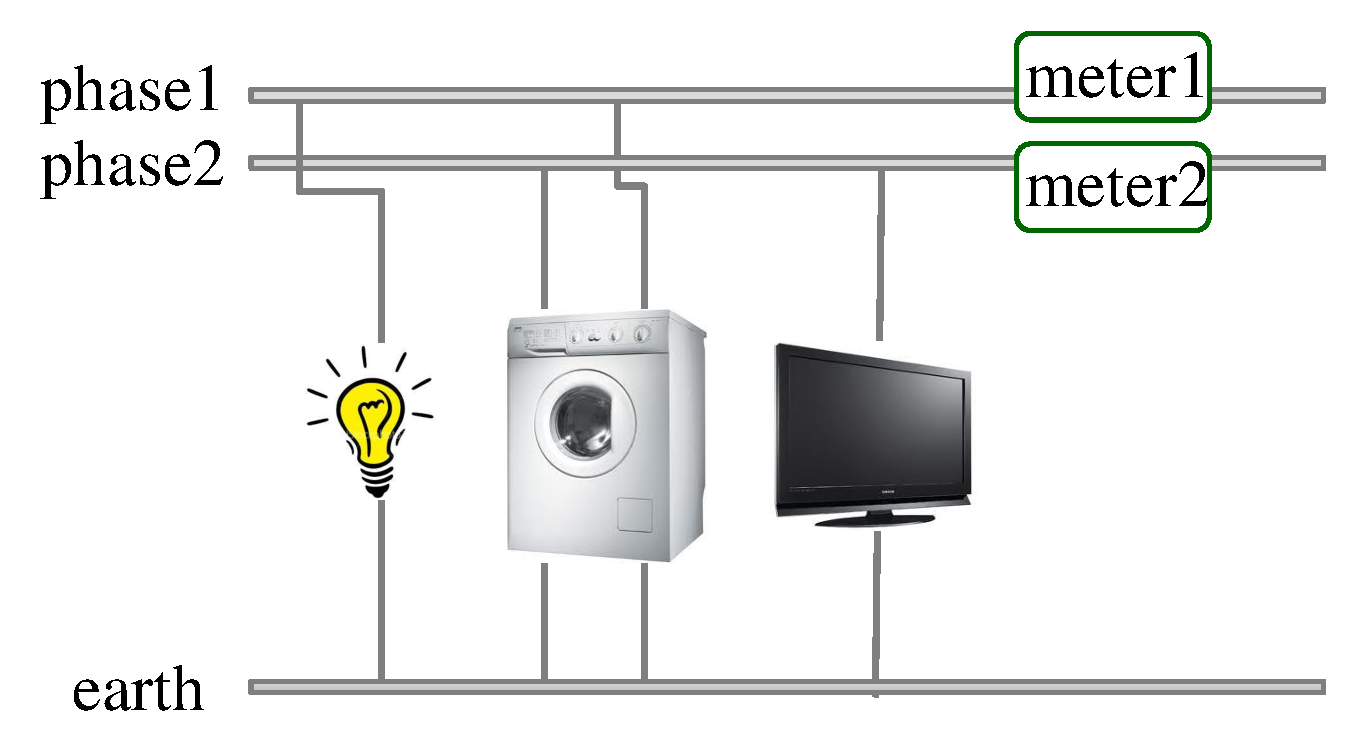
\includegraphics[width=0.5\textwidth]{disaggfigs/background.pdf}
%\vspace{-2mm}
\caption{A residential setup for data collection.}
%\vspace{-2mm}
\label{fig_bg}
\end{figure}

%\vspace{-3mm}
\subsubsection*{High frequency vs low frequency sampling.}
High frequency sampling, typically at the rate of hundreds to thousands of
Hz, can reveal transients in the electrical signal which can then be used as
features for disaggregation. However, customized HW usually needs to be
installed to sample at such high rates.
Low frequency sampling, typically at rates of 1Hz or below, can be obtained
from smart meters, which are being deployed in increasing numbers by utilities
worldwide.

\subsubsection*{Multiple states and transients.}
The device to power state mapping is not one-to-one.
A given device might involve multiple power states
as shown in Figure~\ref{fig_sample} (left).
For instance, a washer/dryer might function at a fixed power level of
1700W but later change levels based on its workload.
Further,
as shown in Figure~\ref{fig_sample} (right), before the refrigerator reaches a
stable state, a transient is observed and,
after a period of time, the power consumption stabilizes to a certain level.

%\vspace{-2mm}
\begin{figure}[!hbp]
\centering
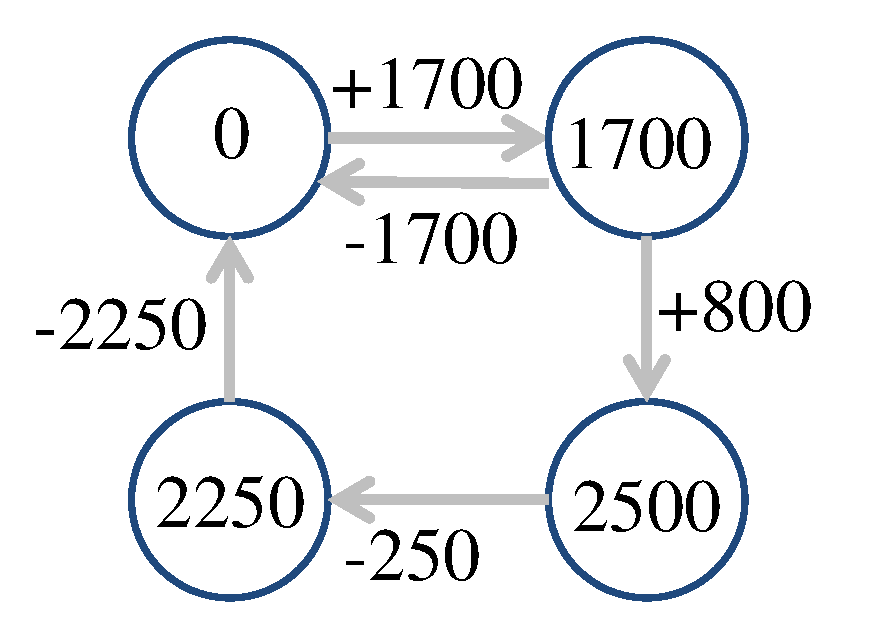
\includegraphics[width=0.3\textwidth]{disaggfigs/washdryer.pdf}
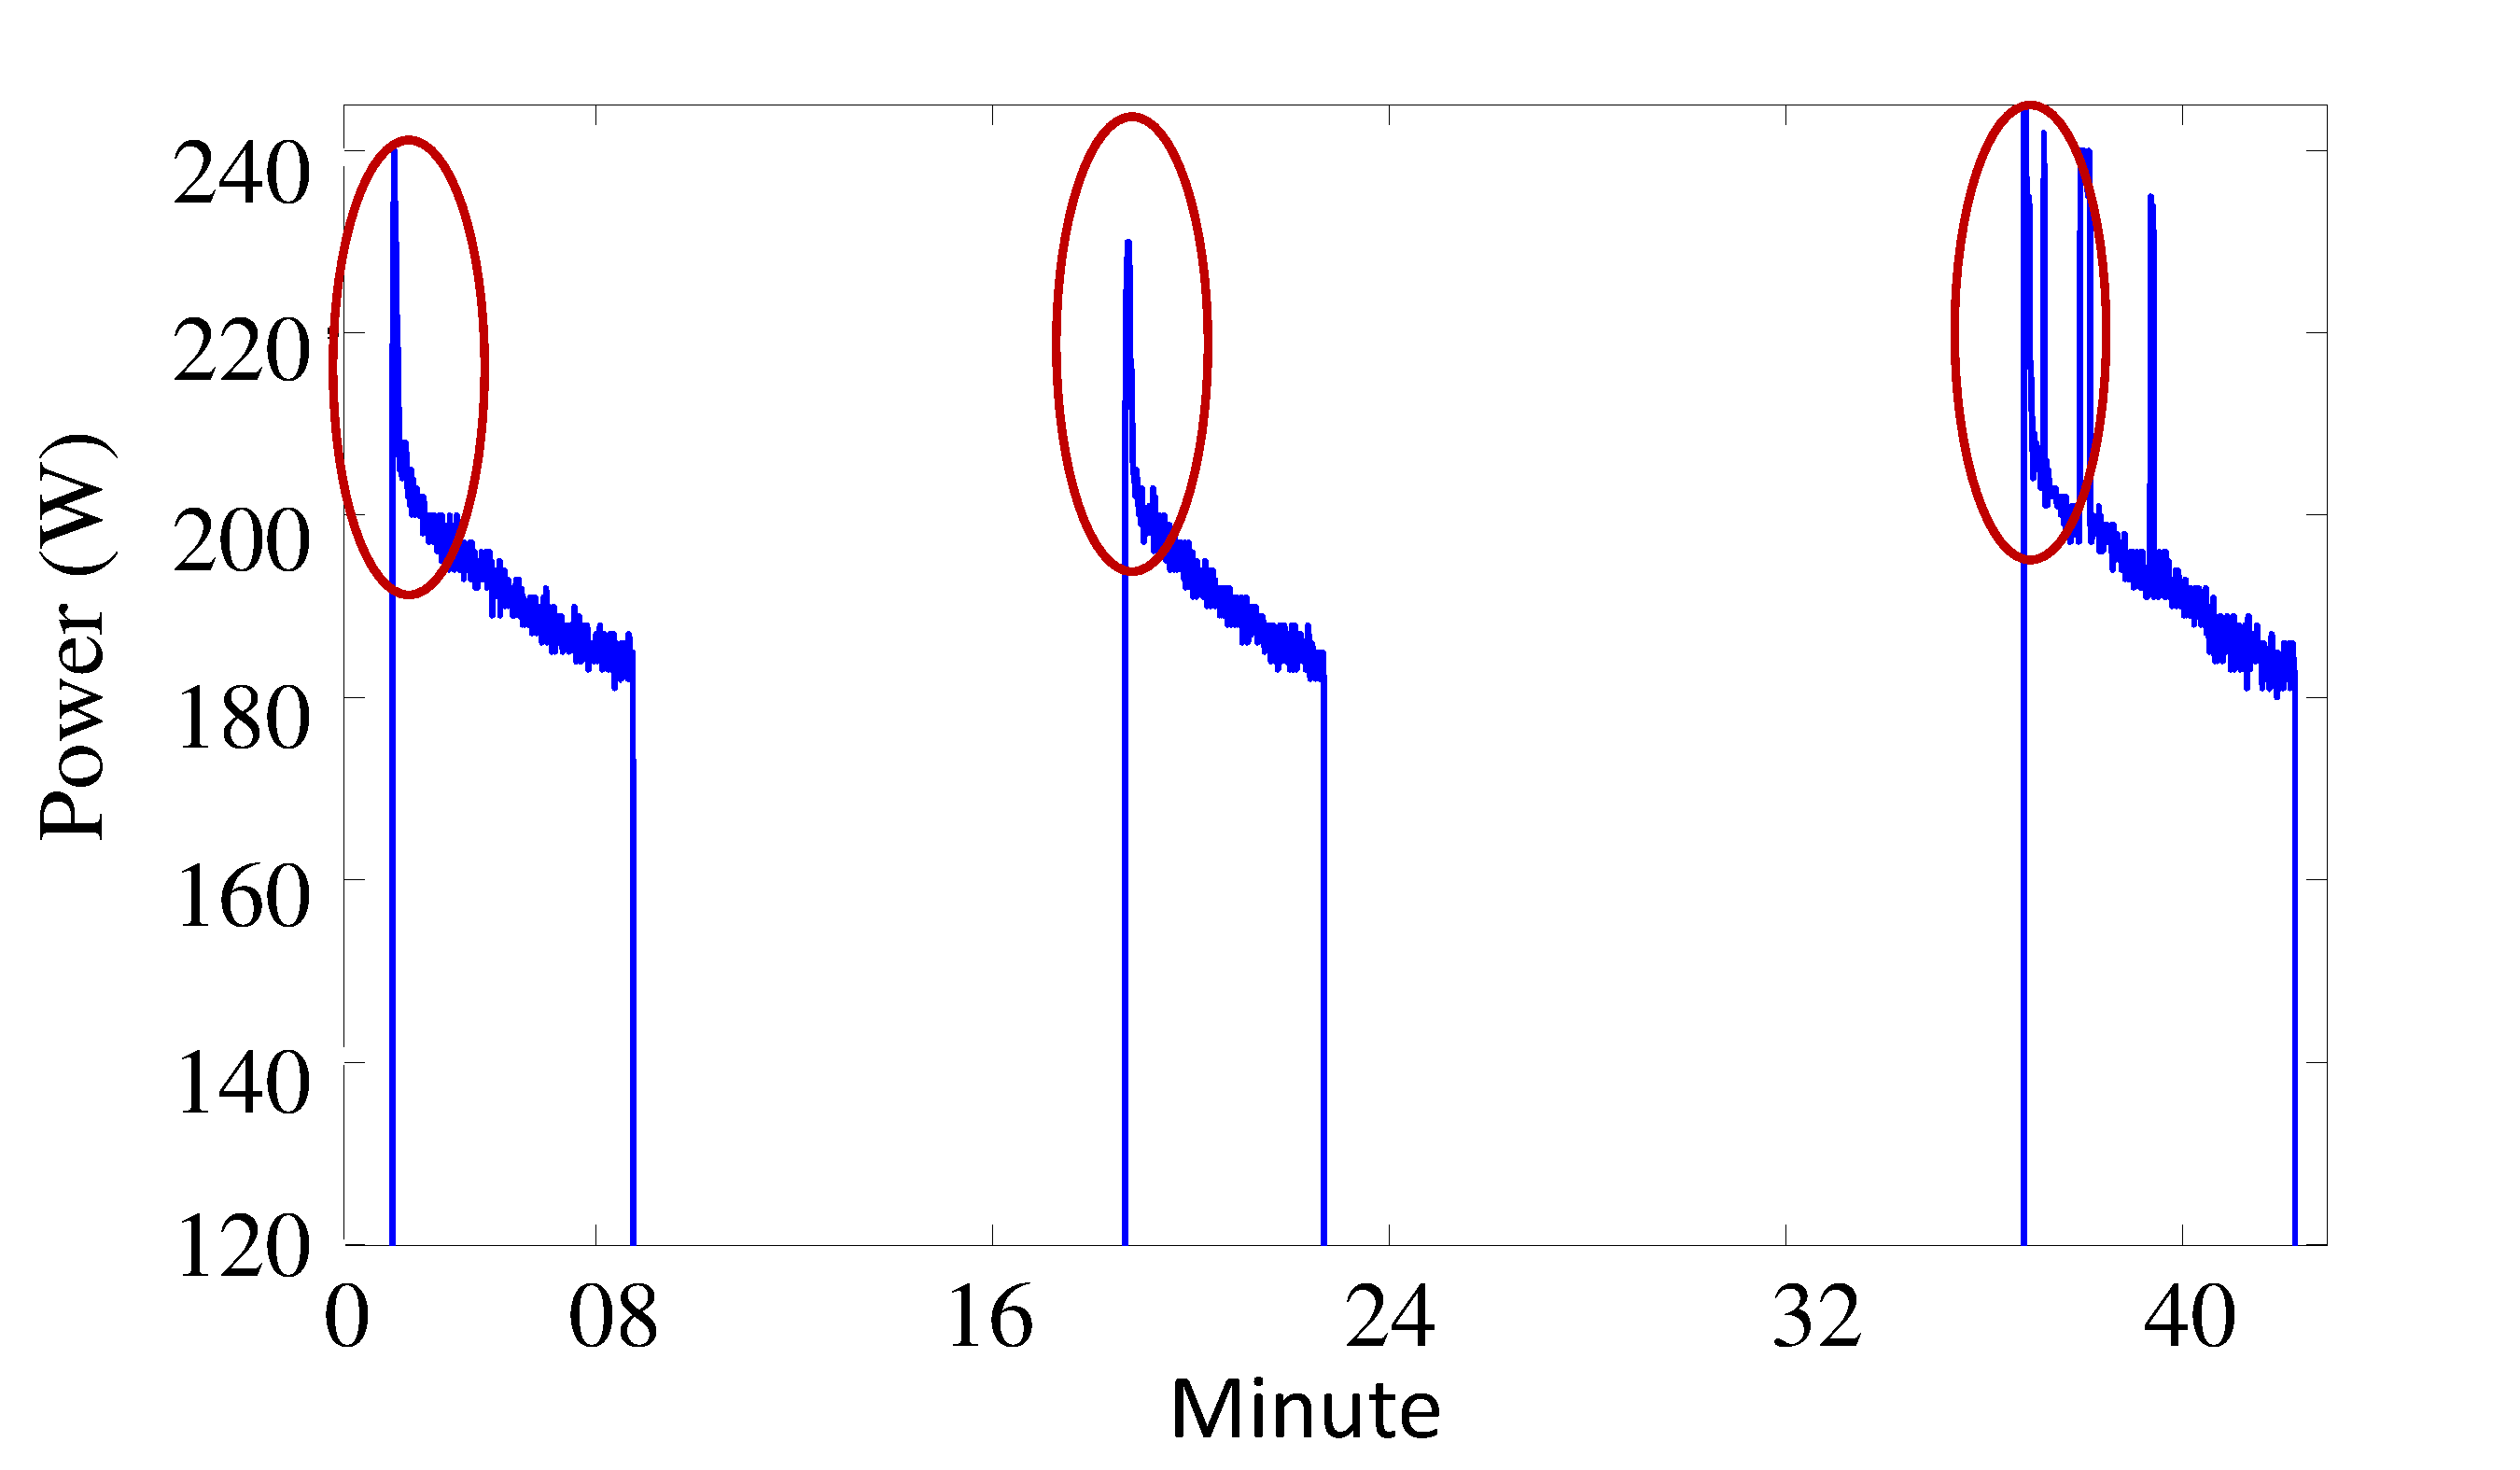
\includegraphics[width=0.7\textwidth]{disaggfigs/refrigerator.pdf}
%\vspace{-2mm}
\caption{Steady state transitions and transient features at startup.}
%\vspace{-2mm}
\label{fig_sample}
\end{figure}

%Electronic devices are very different from its intrinsic characteristics, including
%power consumption magnitude, number of steady states and transient states mode.
%Meanwhile, the working pattern and the operation of a device may affect the usage of
%other devices. By analyzing the aggregated power to extract individual device and
%generalize its usage patterns, we can summarize the power usage pattern
%and then propose better solutions on energy saving.

\subsubsection*{Energy disaggregation.}
Energy disaggregation, initially proposed by \cite{hart1992},
records only the power at the main entry or several points of a building,
and aims to deduce the power consumption of devices in the building over
a period of time through analysis of the aggregate.
Figure \ref{fig_energyDisaggDefinition} gives an example of energy disaggregation
where a total power time series is disaggregated into
fourteen devices over a period of time (here,
8am to 12 noon).
For instance, note that it has been deduced that the refrigerator (in purple)
is switched on for three periods of time, namely,
8:50am to 9:05am,
10:15am to 10:40am, and 11:50am to 12:05pm.

%\vspace{-2mm}
\begin{figure}[!hbp]
\centering
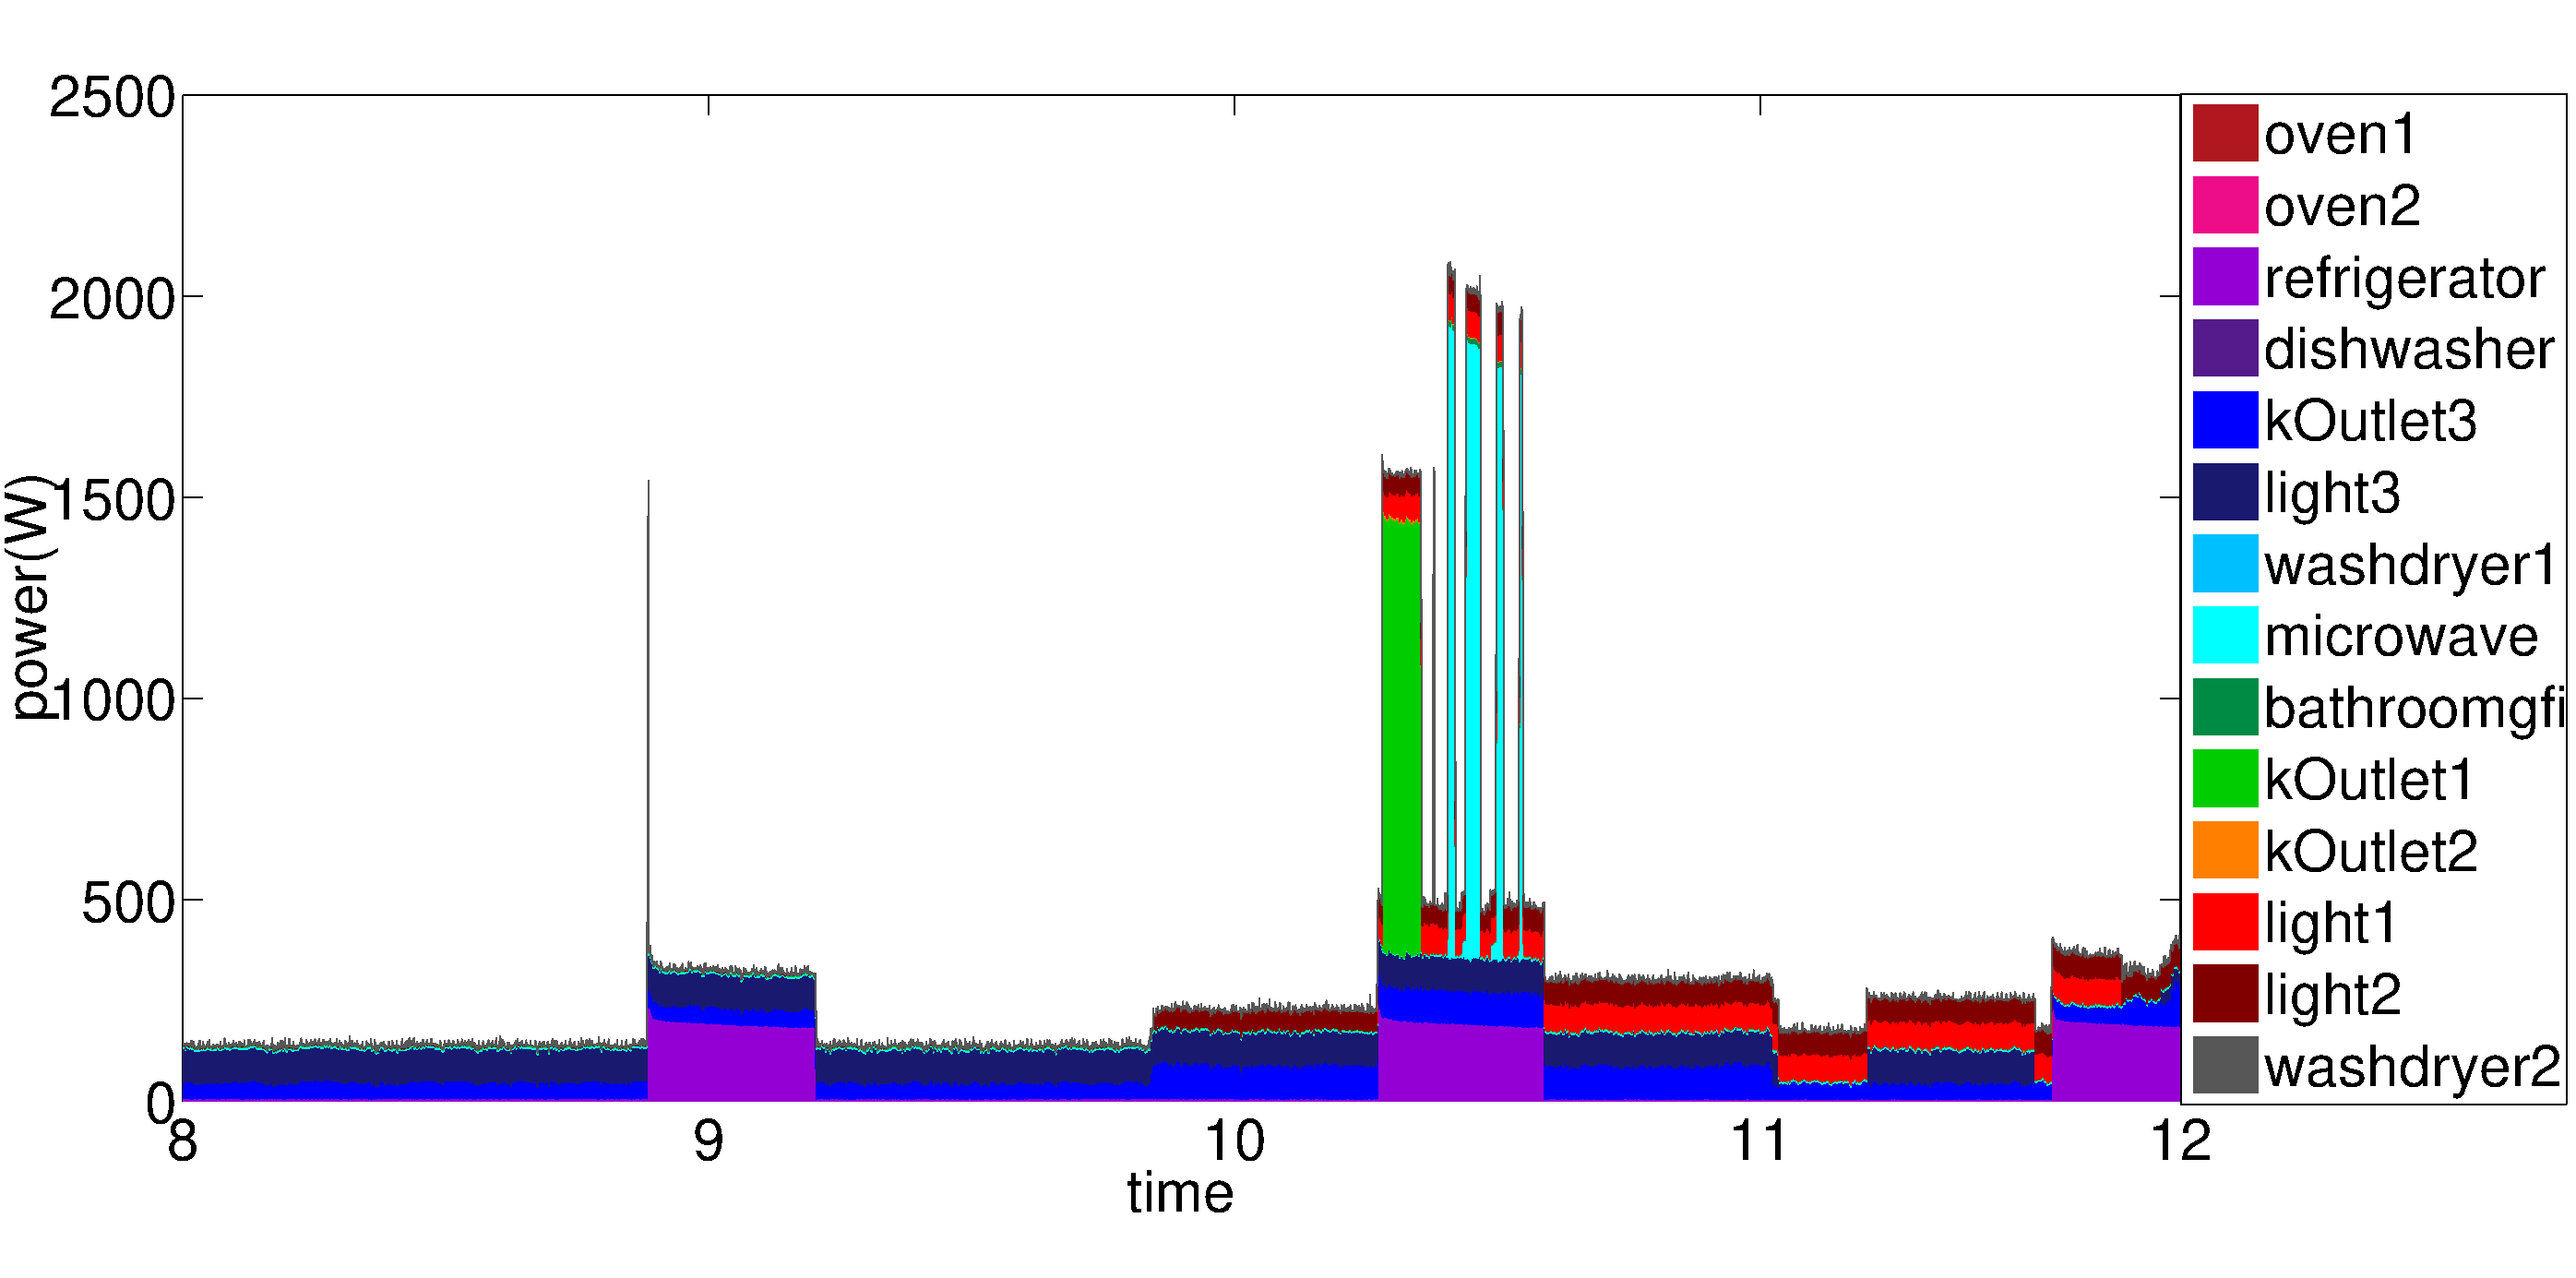
\includegraphics[width=0.97\textwidth]{disaggfigs/energyDisaggDefinition.pdf}
%\vspace{-2mm}
\caption{Example of energy disaggregation.}
%\vspace{-4mm}
\label{fig_energyDisaggDefinition}
\end{figure}
%\vspace{-3mm}


%\vspace{-3mm}
\subsubsection*{Challenges.}
The field of disaggregation has over the last twenty years
 developed many practical solutions drawing primarily from the field of
electrical engineering. However, many challenges remain, including
lack of knowledge about the number of power levels of each device, uncertainty
about the number of steady states for a given device (e.g., a microwave
oven can operate in states of defrost, heat with low power, or with high power),
multiple devices exhibiting the same power level (e.g., lights and monitors),
concurrent switchings on/off of multiple devices (e.g., printers and PCs),
distinguishing start up transients from steady state levels (the former
could persist for significant periods in time in commercial buildings),
variable speed devices that show continuous power levels,
and rare operation of some devices (because they are seldom operated by humans).
These challenges are aggravated
in commercial buildings~\cite{norford1996non}
compared to residential buildings.
%In addition to the above issues,
%\manishc{this is incomplete}

%\section{Related Work}
Most of the approaches that model and predict occupancy primarily use sensor data 
such as room occupancy, use of electrical appliances, water usage, etc.
Several supervised learning approaches like kNN, neural networks, rule-based, 
and Markov chain models have been used to model and predict building occupancy 
\cite{scott2011preheat, alrazgan2011learning, mahmoud2010occupancy, mahmoud2013behavioural, erickson2014occupancy, beltran2014optimal}.  
Using the kNN supervised learning algorithm and monitoring sensor data 
for portion of the day, 
\cite{scott2011preheat} predicts the entire day's occupancy. 
A neural network approach using binary time series based on 
occupancy/unoccupancy along with exogenous input network (NARX) was 
proposed in \cite{mahmoud2010occupancy, mahmoud2013behavioural}. 
Mahmoud et al. tackle the problem by presenting a non-linear autoregressive 
with exogenous input (NARX) network. 
Several Markov chain models like blended Markov chain, 
closest distance Markov chain, 
and moving-window Markov chains were presented in \cite{erickson2014occupancy}. 
A mixture of multi-lag Markov chains was used to predict occupancy of 
single person offices \cite{manna2013learning}. 
In that work, the authors also compare their model with Input Output Hidden Markov Model, 
First Order Markov Chain and the NARX neural network. 

Our work differs from previous research based on the main contributions listed below:
\begin{enumerate}
\item We formulate the problem as one of temporal mining: the activities inside the building are abstracted as episodes, and each episode is connected with an episode generative HMM model.
\item We mine the activity patterns according to the time and gap: both the duration of each type of 
activity, and the gap between two consecutive events are limited in a proper range. 
This range is extracted from the historical data according to the weekday and holidays.
\item Our prediction solution performs better than the kNN approach mentioned before, 
which is generally considered a benchmark in occupancy prediction problem. 
\end{enumerate}

%%%%%comment several paragraphs
\iffalse
These superseded learning approaches are classified into several categories. 
The first is on the probability density distribution of key events. 
\cite{tominaga2012unified} proposes that at a time,  a person goes out has a Bernoulli distribution. 
The second effective benchmark approach is kNN. 
kNN approach is employed in 
\cite{scott2011preheat} to predict the occupancy of the left day 
after knowing the occupancy in the partial day. 
It splits the whole day's time into 96 15-minutes intervals 
then to find the top-5 similar day in the training date. 
The average of these similarity is the predictive occupancy. 
The third is the pattern discovery by rule and neural network. 
A rule-based approach is proposed by
\cite{alrazgan2011learning}  for occupancy prediction under the frame work of Decision Guidance Query Language (DGQL). 
A variant of neural network has been proposed by 
\cite{mahmoud2010occupancy}. \cite{mahmoud2010occupancy} converts the data into binary occupancy/unoccupancy data in the first step. Then a model name non-linear autoregressive network with exogenous input (NARX) network is modeled for prediction. 
\cite{mahmoud2013behavioural} also uses binary time series with NARX network. 
The last are models related to Markov chains. 
Several Markov Chains have been compared in the paper of \cite{erickson2014occupancy}, including blended Markov Chain, closest distance Markov Chain, and the moving window Markov Chain with respect to modeling occupancy. 
\cite{erickson2010occupancy} uses moving-window markov chain for occupancy prediction. 
\cite{erickson2013poem} utilizes the markov chain model and blend markov chain model for prediction. 
\cite{beltran2014optimal} uses a blend-Markov chain model for prediction. 
\cite{manna2013learning} uses mixture of multi-lag Markov chains to predict the occupancy in single person offices. It compares with other previous approaches Input Output Hidden Markov Model, First order Markov Chain and NARX Neural Network. 

This work contributes the follows:
1) formulate the problem as a temporal mining problem;
2) mine the activity patterns according to time and gap;
3) the occupancy prediction performance of this temporal mining approach works better than kNN for most cases.
\fi


%\vspace{-1mm}
\subsubsection*{Features from meters.}
Let us first review the type of features discernible from metered usage data.
From low frequency measurements, it is possible to infer features such as
steady states, real power, reactive power,
low-order harmonics, and the time of day.
From high frequency measurements, in addition, we will be able to discern
characteristics
such as higher-order harmonics and the current or voltage waveform.
In addition, from high frequency data, it is possible to discern transient states.


%\vspace{-1mm}
\subsubsection*{Prior approaches to disaggregation.}
Initial research focused on using
simple device features such as real power
and reactive power~\cite{hart1992}.
With the development of automated meters,
transient states generated when devices turn on have been
employed to
identify devices \cite{shaw2000PhdThesis}.
Raw current waveforms \cite{srinivasan2006neural},
and voltage waveforms \cite{lam2007novel},
and transforms of the current waveform \cite{chan2000harmonics}
have also been adopted as characteristics. In particular,
harmonics of non-linear devices
have been utilized in prior work \cite{chan2000harmonics}.
Further, non-AC power features such as power line noises \cite{patel2007flick},
time of day and device correlations \cite{kim2011unsupervised},
can be combined with AC power features to aid disaggregation.
The underlying algorithms have been drawn from a variety of domains:
supervised learning~\cite{nakano2007non},
data mining, optimization, and signal processing, e.g.,
kNN \cite{shaw2000PhdThesis},
SVM \cite{patel2007flick},
%Neural Netowork \cite{roos1994using},
%Genetic programming \cite{baranski2004genetic}, and
sparse coding \cite{kolter2010sparse}. Recent research has placed a great
emphasis on
building in unsupervised learning features, including
hierarchical clustering \cite{lam2007novel},
semi-supervised approaches~\cite{parson2012nonintrusive},
factorial HMMs \cite{kim2011unsupervised}, and
AFAMAP \cite{kolter2012aistat}.
%In addition, there's semi-supervised approach \cite{parson2012nonintrusive}.
%Some optimization algorithms such as dynamic programming \cite{baranski2004detecting} and
%viterbi algorithm \cite {zeifman2011viterbi}.
%Signal processing algorithm wavelet transform \cite{chan2000harmonics} is
%applied with electricity feature.

%In prior work, some papers have already summarized the
%features and algorithms in \cite{zeifman2011nonintrusive}
%and \cite{liang2010load}.
%They emphasize on the electrical engineering area and
%ignore basic conceptions on the background knowledge.
%The contribution of this survey is that
%it gives a brief introduction of energy disaggregation
%from from the perspective of data mining.
%Energy disaggregation is only a part of energy saving.
%The techniques it uses can also be applied to
%water disaggregation \cite{dai2011multi} and
%gas disaggregation \cite{froehlich2011disaggregated}.


%There has been renewed interest in energy diaggregation or Nonintrusive
%Appliance Load Monitoring (NIALM) in recent years given the increasing
%cost of energy and concern over climate change. Energy disaggregation was
%first presented in the seminal work of Hart \cite{hart1992}. He described how
%features, such as, differences in real and apparent power in a whole house
%power measurement, could be used to identify the turning ON/OFF of individual
%appliances. He also proposed use of finite state machines to develop
%identifying signatures for complex appliances with multiple power states.
%
%Disaggregation approaches can be mainly categorized based on the features used
%and whether it is supervised or unsupervised. Most approaches in the past have been
%supervised \cite{hart1992,norford2006,shwetakpatel2007,berges2010,kolter2010redd},
%where a labeled data set (ground truth) is used for
%training. However, creating such a data set is error-prone, laborious and
%intrusive, which convinced us to not  pursue a supervised
%approach in our work.
%
%Recently, some unsupervised approaches have been proposed,
%where labeled data is not required. Kim et al. \cite{kim2011unsupervised} proposed
%extensions to factorial hidden markov models to include additional features
%such as time of day and dependency between appliances. Zico et
%al. \cite{zico-aistat2012} use a difference factorial hidden Markov model, and
%develop a novel approximate inference procedure, which they call AFAMAP
%(Additive Factorial Approximate MAP).
%
%Features used for disaggregation can be classified into stable state and
%transient features.  Transient signatures capture electrical events, such as
%high frequency noise in electrical current or voltage, generated as a result
%of an appliance turning on or off. Although these features are good candidates
%for use in disaggregation, sampling data fast enough to capture them requires
%special instrumentation. For example, Patel et al. use a custom built device
%to measure at rates up to 100KHz \cite{shwetakpatel2007}. However, most smart
%meters deployed in the U.S. have low sampling rates, typically 1Hz or less.
%Stable-state signatures relate to more sustained changes in power
%characteristics when an appliance is turned on/off. These persist until the
%state of the appliance changes, which can be captured with low frequency
%sampling. But even for stable-state features, the frequency of sampling is
%important since at low sampling rates the probability of multiple on/off
%events occurring between two measurements increases, making the disaggregation
%task more difficult.

%\input{Formulation}

%\vspace{-2mm}
\section{Temporal Motif Mining}
Early approaches to disaggregation (e.g., Hart\cite{hart1992})
assume that only the
aggregated current and voltage information is known whereas
later work assumes that the number of devices, possible steady states
of devices are also known,
so that the problem reduces to minimizing the error between
the combination of disaggregated devices and the ground truth devices.
Here, we assume that the number of devices/number of circuits is known,
a reasonable assumption since such information is obtainable from a top-level
circuit map of the building.

%\input{Framework}
%\section{Framework}
Our framework (see Figure~\ref{fig_fw})
unifies clustering and temporal data mining
to discover power levels,
forms episodes from power levels corresponding to devices,
and models the underlying time series as a mixture model whose components
correspond to the device episodes.
The framework has six key stages, viz.
baseline removal,
steady states extraction,
episode mining and selection,
probabilistic sequential mining,
motif mining or time-based motif mining, and
device recovery.
Gray box in Figure~\ref{fig_fw} denotes that the step can be neglected
(and are typically used when disaggregating for commercial buildings).
%\manishc{ungray baseline removal}

%\vspace{-3mm}
\begin{figure}[!hbtp]
\centering
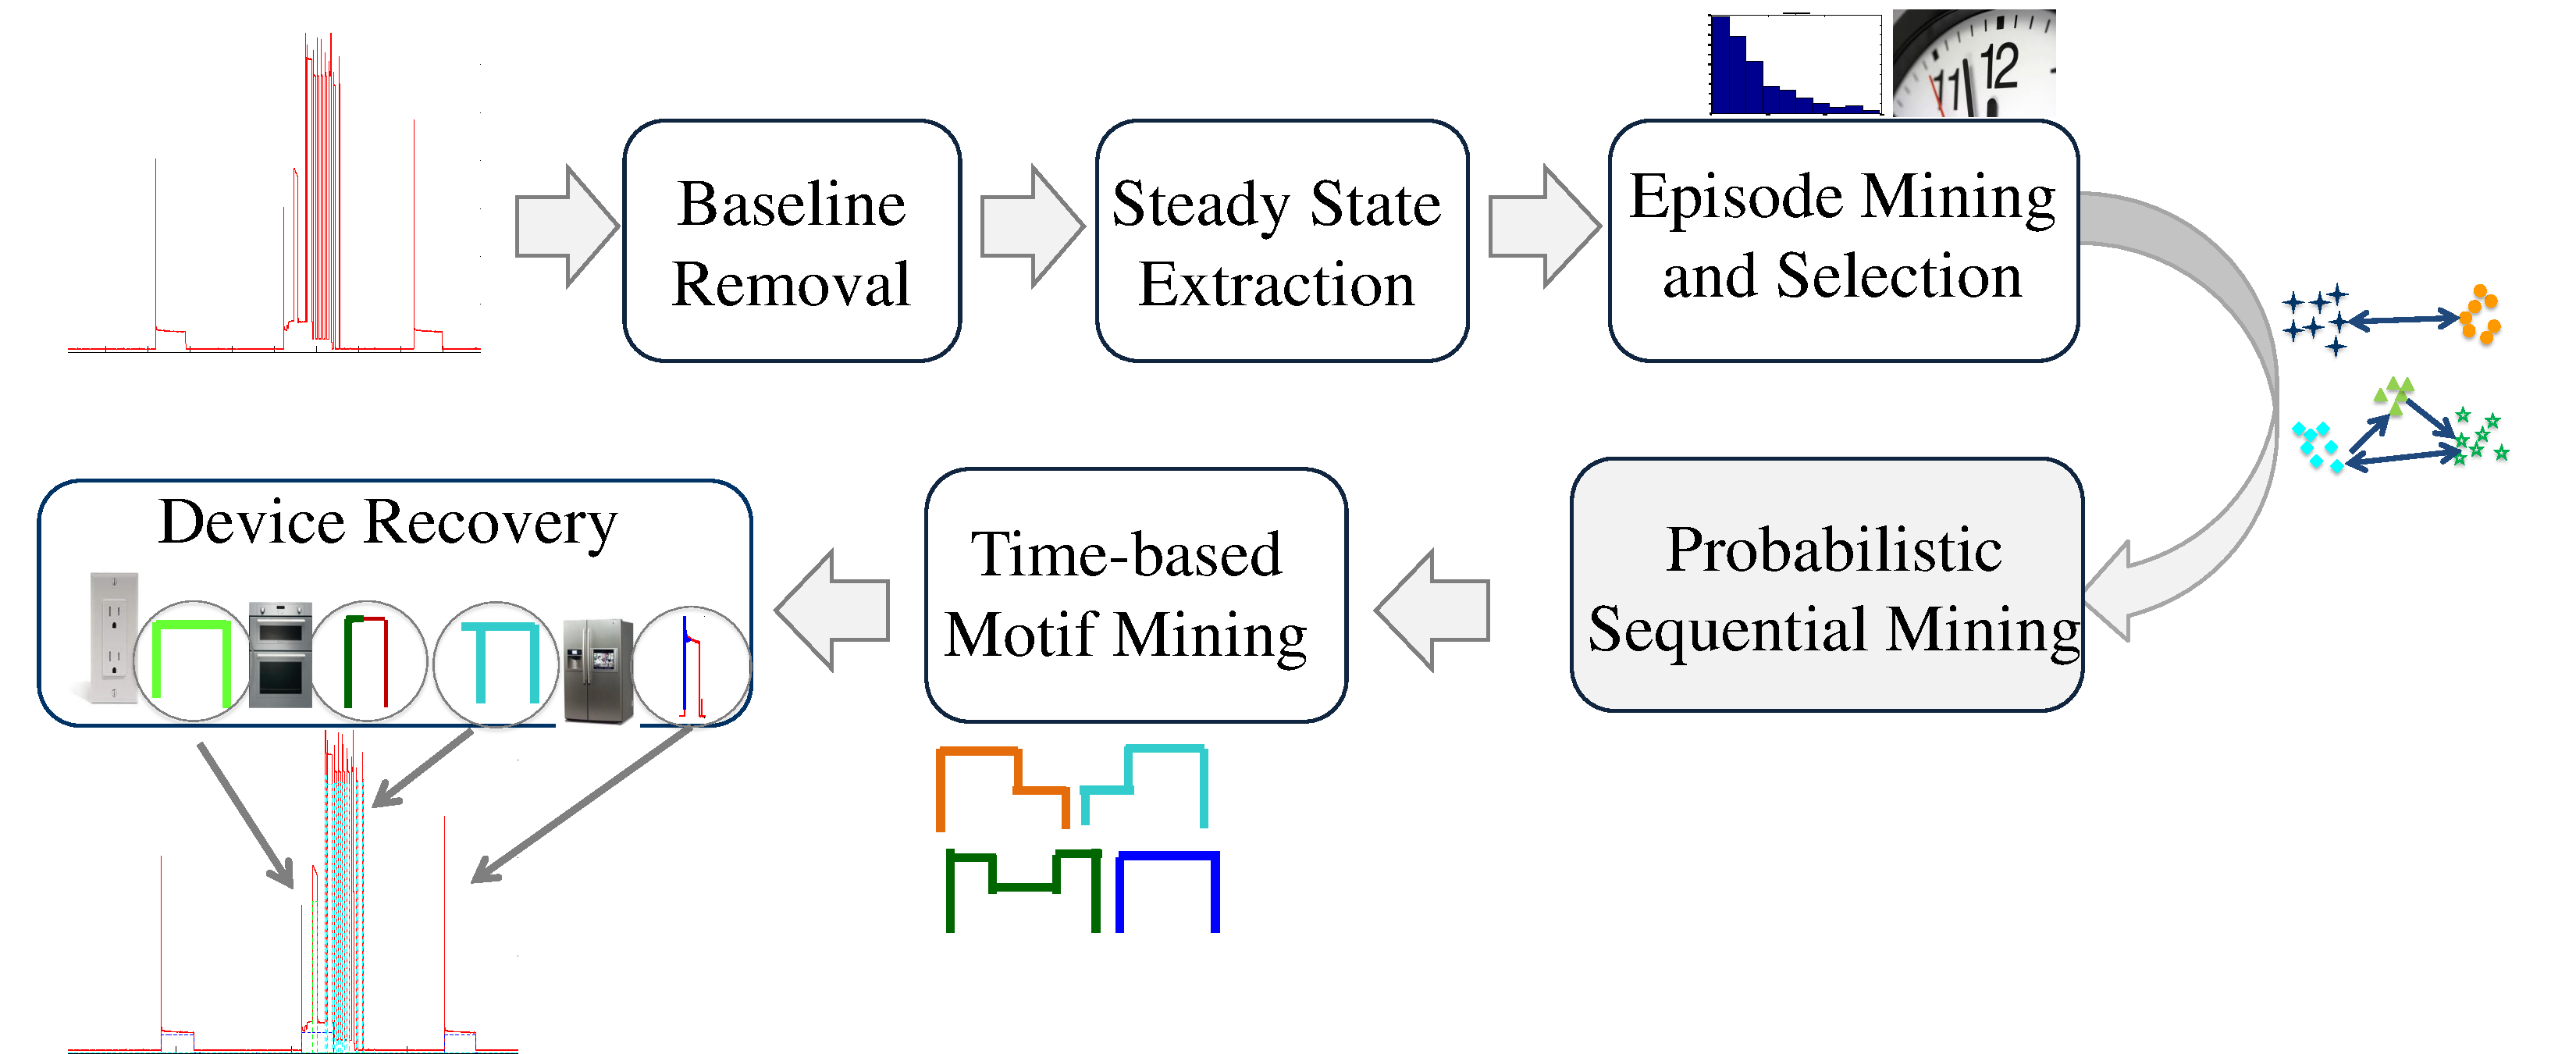
\includegraphics[width=0.97\textwidth]{disaggfigs/arch.pdf}
%\vspace{-3mm}
\caption {Temporal motif mining framework for disaggregation.}
%\vspace{-3mm}
\label{fig_fw}
\end{figure}

\subsubsection*{Baseline extraction.} Baseline removal
%, typically
%necessary in commercial buildings,
aims to separate devices that are
always on. Given the aggregated (input) power series $P(t)$ over time period $T$,
the baseline power $P_\textrm{base}$ is defined such that
$P_\textrm{base} \ge \min_{t} P(t)$ and where
$f(P_\textrm{base}) \ge \alpha T$ (a minimum support threshold).
%%\narenc{I am not
%sure this next sentence is correct, or what it exactly means. Huijuan, can you
%clarify? Manish, can you help rephrase or remove?} If we view
%the baseline power as having been produced by a virtual device, then it is easy
%to show that any further drops in power below $P_\textrm{base}$ must also
%come from the virtual device.

\subsubsection*{Steady state extraction.} Two basic approaches here
involve a heuristic method (window-sized filtering) and the more systematic
Dirichlet process Gaussian mixture models (DPGMMs)~\cite{gorur2010dirichlet}.
In the former, a mean filter smoothing is typically applied
whose window size is adjusted to correspond to the mean or maximal start
time duration in the given collection of devices (e.g., this could be just a second
in the case of lighting, but higher for say a refrigerator).
A DPGMM can be viewed as an infinite-mixture extension of a traditional
Gaussian mixture model (GMM). Recall that in a traditional GMM,
${\bf y}= \Sigma^{k}_{i=1} \alpha_i N(\mu_i, \Sigma_i)$ where
$\Sigma_i \alpha_i =1$, and
each component has a mean $\mu_i$
and covariance matrix $\Sigma_i$. A DPGMM defines Gaussian priors for all
the component means $\mu_j$:
\begin{displaymath}
p(\mu_j|\lambda, r) \sim N(\lambda, r^{-1})
\end{displaymath}
The distribution of $\lambda$ is set to be a Gaussian prior
and the distribution of $r$ is set to have a Gamma prior, so
that the number of points in each component
$i$ conforms to a multinomial distribution with an unknown number of
components. After modeling all the power levels in this manner, we
replace all values with their representative (nearest centroid) power levels,
record only the differences in successive power levels, and use this
`diffs' time series for further modeling.

%\vspace{-3mm}
\begin{figure}[!hbtp]
\centering
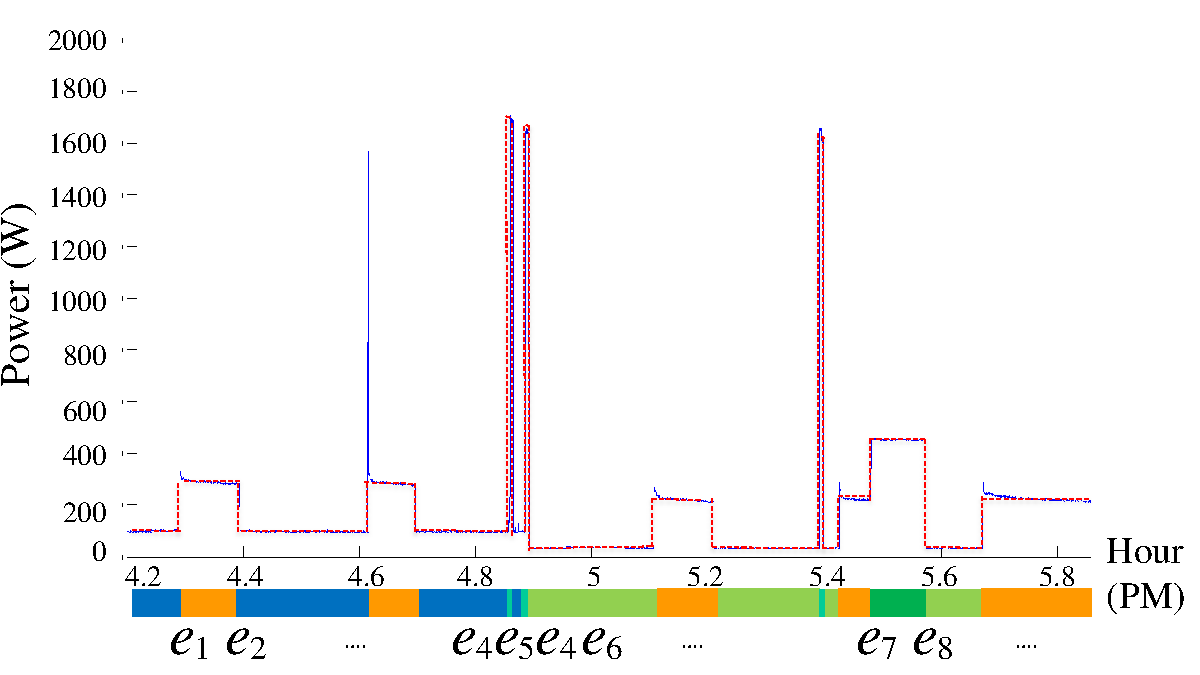
\includegraphics[width=0.93\textwidth]{disaggfigs/steadyevents.pdf}
\caption{Mining episodes from a symbolic time series.}
\label{fig_tevents}
\end{figure}
%\vspace{-3mm}

\subsubsection*{Episode mining and selection.} The goal of episode mining~\cite{motifgoal}
is to identify repetitive sequences of power level changes and, further, to
isolate (select) those episodes that potentially correspond to the operation
of a single device. Recall that at this point, we have generated a
symbolized time series from the `diffs' data. Let the set of symbols be S.
From the diffs sequence, the transitions between
symbols are recorded to help constitute episodes. We set the max
episode length to be N, corresponding to the N-1 states of a device. Then all
the symbols in the symbol set are permuted with length from 2 to N. As a
result, all possible episodes with length from 2 to N are generated. To select
valid episodes, some constraints checks are performed.

First, steady
state values extracted from the previous
step are clustered into a discrete symbol time series and transitions between
symbols are recorded to identify episodes.
Figure~\ref{fig_tevents} describes how transition events are generated,
resulting in the event series:
$(e_1, e_2, e_1, e_2, e_4, e_5, e_4, e_6, e_1, e_2, e_4, e_5, e_1, e_7, e_8, e_1)$.
An episode of length $N$,
$E=(e_1 \rightarrow e_2 \rightarrow...e_N)$,
denotes an ordered sequence of (not necessarily consecutive) symbols.
To select those episodes that correspond to characteristics of an electrical device,
several constraints are introduced:
\begin{enumerate}
\item {\it The sum of the power level changes corresponding to
the events of a episode is nearly zero.}
%In other words, for a K-length episode \begin{math}(e_0, e_1, ..., e_K) \end{math}
%\begin{displaymath}
%\sum_{i=1}^{K}e_i < { \alpha \times max\{e_0, ..., e_K\}+ \beta}
%\end{displaymath}
%For any device, it starts from zero,
%then experiences a series of power changes
%finally goes to zero power consumption.
%In practice, the sum of a episode is not strictly
%zero because for any steady power consumption level,
%it has some range.
%For the discrete power consumption devices,
%the power consumption level usually
%conforms to Normal distribution instead of one fixed value.
Figure~\ref{fig_sample} (left) shows an example, where there
are two complete episodes for a washer-dryer:
(+1700, -1700) and (+1700, +800, -2250, -250).
\item {\it The sum of the power level changes corresponding to any
prefix of a episode is positive.} This constraint is particularly geared
toward multiple state devices.
Fig~\ref{fig_cst} shows two examples of episode selection
based on this constraint
The episode (+100,-100) is retained but the episode (-100,+100) is discarded.
As another example, episode (+600, -400, +1000)
is chosen and episode (+600, -1000, +400) is discarded. Note that this assumes
there are no always on devices.

%\vspace{-3mm}
\begin{figure}[!hbtp]
\centering
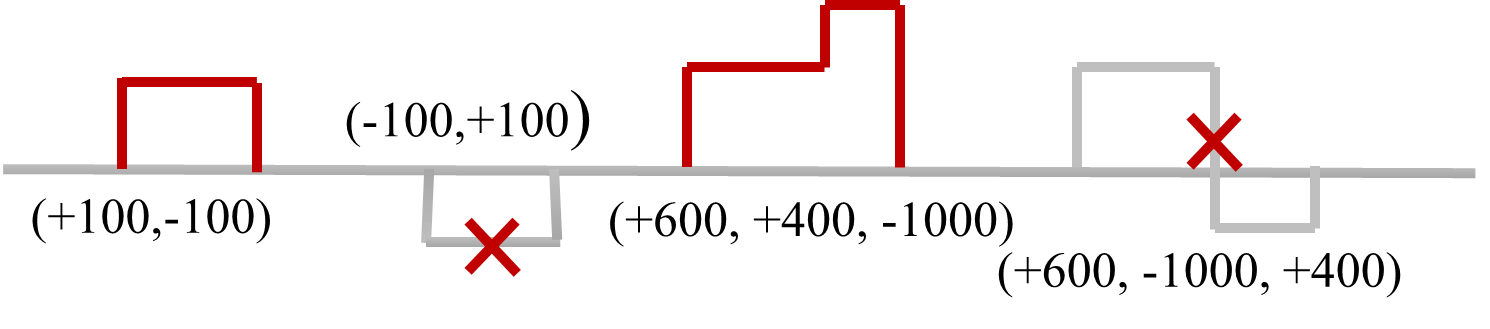
\includegraphics[width=0.7\textwidth]{disaggfigs/cst.png}
\caption{Episode constraints.}
\label{fig_cst}
\end{figure}
%\vspace{-3mm}


\item {\it The absolute value of the power level of any event in an episode
related to a device
must be higher than a support threshold over the maximum level in the
episode.} In other words, power state changes in a device are assumed to be
greater than a support threshold.
This condition is intended to exclude cases where the low power consumption of
one device inadvertently forms part of the episode of a high power consumption
device. For instance, using a support threshold of $0.1$, the episode
$(1000,-850,-90)$ will get disqualified (because $90 < 100$) since
this episode is likely generated by more than one device, rather than
a single device.
\end{enumerate}

\subsubsection*{Probabilistic sequential mining.} This step aims to
discover devices that exhibit several power levels sequentially and which
operate frequently within a very short period of time.
We use sequential mining~\cite{srikant-agrawal}, a levelwise framework,
with duration constraints to discover such devices. We begin
by seeking episodes that satisfy the
above three checks and which can be systematically grown into longer chains
of power level changes within a user-specified window.
%Some device in commercial buildings uses power
%very frequently in a very short of time.
%In order to connect an episode with this kind of
%device, we cluster the power level diffs
%according to the operation hour, weekday to
%form an episode.

%\narenc{What is probabilistic in this?}
%\manishc{how is this different from the next step? and where does the
%hierarchical clustering using time of day, day of week belong}
%\huijuanc{the following is added by huijuan}
Devices in commercial buildings
are often scheduled to turn on/off at fixed time.
Therefore, we cluster power levels according to time of day and
day of week.
We apply hierarchical clustering with Ward Euclidean distance
to diffs of power levels.
As a result, each set of power level diffs
that qualifies the three constraints are chosen.
For example, a cluster can identify a power level diff set $S=\{e_1, e_2, ...e_n\}$
belonging to a single device.

Regarding probabilistic sequential mining,
a coverage probability $\theta$, say 0.9, is introduced
to determine what percent of power levels
should be covered for each device.
Probabilistic sequential mining only considers the
coverage of power levels rather than
the sequence of power levels as motif mining.

\begin{figure}[!hbtp]
        \centering
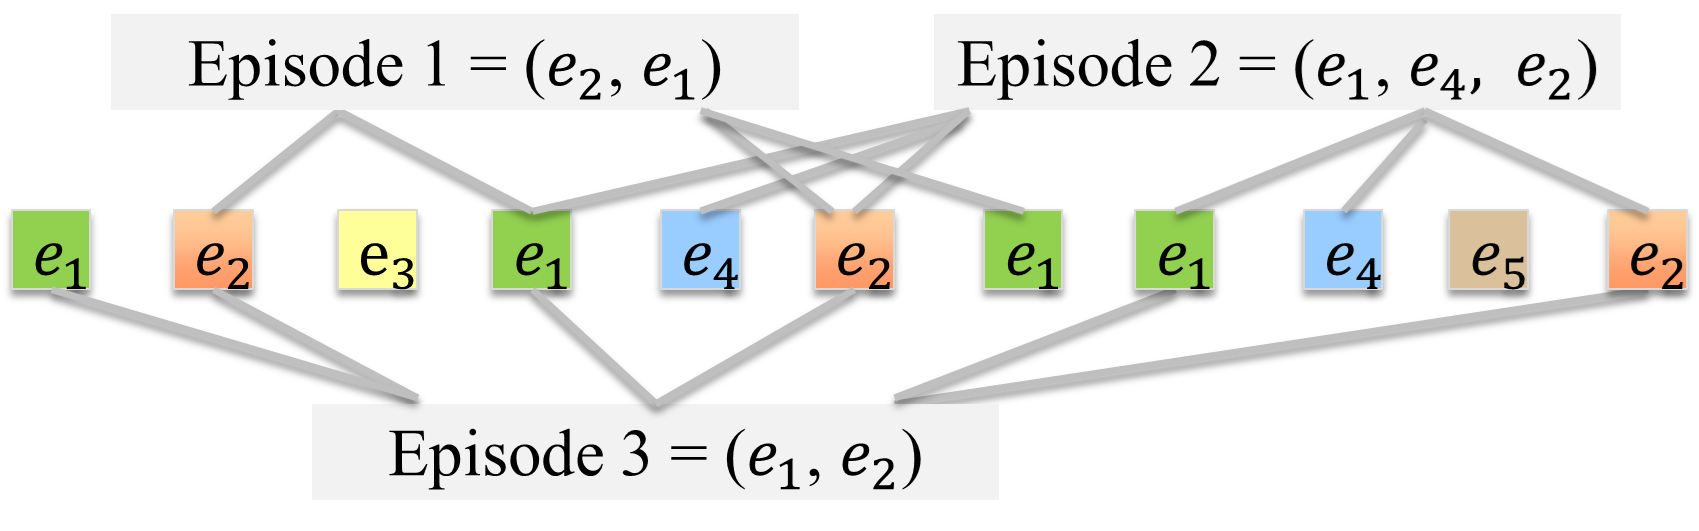
\includegraphics[width=0.67\textwidth]{disaggfigs/motifSample.png}
        \caption{Illustration of motif mining. Note that there are 3 non-overlapped
occurrences of Episode 3.}
        \label{fig_motifsample}
\end{figure}


\subsubsection*{Motif mining.} Motif mining aims to find repetitive
episodes in a time series using the technique of non-overlapped
occurrences~\cite{vatsan-paper}. Assume
there are five power event change symbols \begin{math} \{e_1, ..., e_5\} \end{math}
and a time series \begin{math} (e_1, e_2, e_3, e_1, e_4, e_2, e_1, e_1, e_4, e_5, e_2) \end{math}
which is produced by these five symbols as shown in Figure~\ref{fig_motifsample}.
Consider the episode Episode 3, composed of
two ordered events $(e_1, e_2)$.
In this time series, there are four \begin{math}e_1 \end{math} and
three \begin{math}e_2 \end{math} occurrences, and three instance of Episode 3.
The first \begin{math} e_1 \end{math} and first \begin{math} e_2 \end{math} comprise
the first instance of Episode 3.
The second \begin{math}e_1 \end{math} and second \begin{math}e_2 \end{math} make up
of the second instance of Episode 3.
The third instance is composed of the fourth \begin{math} e_1 \end{math} and
the third \begin{math} e_2 \end{math}.
Other possible instances of Episode 3 which may cause overlaps with the above
instances are not considered in the non-overlapped count measure,
such as \begin{math} (e_1, e_2) \end{math}
which consists of the first \begin{math}e_1 \end{math} and the
second \begin{math}e_2\end{math}. With this count measure, all episodes
that have support greater than the specified threshold are discovered
by motif mining.
For commercial buildings that have scheduled on/off devices, we
adopt a time-constrained version of non-overlapped count, where the episode
growth is restricted to events that fall within a specified time window.

%\subsubsection*{Device recovery.} The final step is to correspond each of
%the reconstructed episodes with one device.

\subsubsection*{Computational complexity} Assume $m$ is
the number of power levels in the `diffs' data. Then the computational complexity of
DPGMM is $O(mnd^2+md^3)$, where $n$ is the number of points in diffs data,
and $d$ is the number of feature dimensions (e.g.,  time, date).
The computational complexity
for the episode generation step is $(p-1)O(m^2)$, where $p$ is the
maximal
episodes length. Since $p$, which is 3, and $m$, which is 14 or 27, are small,
we apply a brute force approach. The worst-case time complexity of the motif
mining algorithm is $O(msq)$, where $q$ is number of candidate episodes, and
$s$ is the size of the episode.

\subsubsection*{Parameters} There are three kind of parameters used:
(1) those pertaining to power level generation, (2) threshold for moitif
mining, and (3) window size for median filtering. For each of these, a range
of values were tried and their values were set based on performance on a test
set.
%This will be detailed discussed in the appendix.

%\section{Evaluation Metric}
\label{sec:evaluation}
To the best of our knowledge, there is no unified evaluation metric to evaluate the
disaggregated results of energy disaggregation.
Suppose we know the true power consumption value of each device, then there are two 
metrics to evaluate the  device disaggregation results - event based and time 
series based. In the event based metric, we check whether the 
disaggregated turning on and off events are correctly classified for the target device. 
The time series metric gauges whether the disaggregated power values of each device 
is in the range of ground truth over a period of time. 

For both event-based metric and time-series-based metric, 
the disaggregation results can be measured through the confusion matrix, 
F-measure, or simple error rate. 
 
%We introduce precision, recall, and F-measure to evaluate it.
%In classification, true positive (TP) means the result is correct;
%false positive (FP) means the unexpected result; 
%true negative (TN) means the missing results; 
%and false negative (FN) means the correct absent values.
%Precision is to calculate for the disaggregated energy,
%how much is correct. Recall is to calculate how much
%energy is identified.
%The precision and recall are calculated as Equation (\ref{eq_precision}) 
%and Equation (\ref{eq_recall}). 
%\begin{equation}
%\label{eq_precision}
%precision=\frac{TP}{TP+FP}
%\end{equation}
%\begin{equation}
%\label{eq_recall}
%recall=\frac{TP}{TP+FN}
%\end{equation}
%F-measure value is the harmonic
%mean of precision and recall.
%\begin{equation}
%\label{eq_fmeasure}
%F-score= 2 \times \frac{precision \times recall}{precision + recall }
%\end{equation}

%The evaluation metric includes the events classification error rate
%\cite{patel2007flick} and time point-to-point energy comparison \cite{kolter2012aistat}.

%\begin{table}
%\tbl{Evaluation Metrics \label{tb_evaluation}} {
%\begin{tabular}{|c|c|c|}
%\hline
%& events & time series\\
%\hline
%taxonomy & set classification & point-to-point \\
%\hline
%F-measure & TP,FP,TN,FN for events & TP,FP,TN,FN for each energy value \\
%\hline
%error rate & event is classified into right device & for each data point, the value is classified right \\
%\hline
%\end{tabular}}
%\end{table}
%The events includes real power changes events,
%real power and reactive identification events,
%transient shape events and so on.

\subsection{Evaluation Based on Events}
Event-based evaluation metric, primarily on and off events, has been widely used in 
previous research work. 
They are identified by real power and reactive power as stated in~\cite{berges2009learning} and~\cite{chang2010newmethod},
by real power and transient shapes~\cite{froehlich2011disaggregated},
by real power, reactive power and voltage-current trajectory~\cite{yang2007design},
by just transient shapes~\cite{chang2008load},
by comparing the waveforms as shown in~\cite{suzuki2008nonintrusive} and~\cite{berges2010enhancing},
or by analyzing the voltage noise~\cite{patel2007flick}.
%No matter which feature is adopted and
%which algorithm is applied,
%the target is to improve the
%event classification accuracy.

Generally, the events classification rate is
calculated as follows.
For each device,
suppose there are totally $N$ on or off events 
$\{E_1, ..., E_i, ..., E_N\}$ during
a period of time,
the corresponding predicted events are
$\{\hat{E_1}, ..., \hat{E_i},...,\hat{E_N}\}$,
and the the coverage range of these on or off events is
given in Equation (\ref{eq_eventEvaluation}) in~\cite{nakano2007non}.
\begin{equation}
\label{eq_eventEvaluation}
E_{coverage} = \frac{\sum_{i=1}^N (E_i - \hat{E_i})}{\sum E_i}
\end{equation}
Higher coverage for a device implies better prediction results.

%In order the improve the classification accuracy,
%\cite{gupta2010electrisense} and \cite{onoda2000applying}
%trains data by cross-validation.


%Equation.\ref{eq_eventEvaluation} according to devices
%over the test time period.
%This time period can be specified by users.
%\cite{kolter2010sparse} evaluates the results with one-week's
%accumulated data.
%\begin{equation}
%Accurage \equiv \frac{\sum_{i,q}\min\{\sum_p(X_i)_{pq}, \sum_p(B_i\hat{A}_i)_{pq} \}}{\sum_{p,q}\bar{X}_{p,q}}
%\end{equation}

Secondly, the disaggregation accuracy rate
can be calculated by judging whether
the disaggregated devices are classified as the
right device or not.~\cite{gonccalves2011unsupervised} evaluates the classification results
based on this criteria as given in Equation (\ref{eq_clusterEvaluation}).
\begin{equation}
\label{eq_clusterEvaluation}
purity_m(\Omega, C) = \frac{1}{1/N_m}\sum_k \max_m |\omega_k \subset c_m|
\end{equation}
where $\Omega$ is the set of all ground truth device labels,
$C$ is the disaggregated device labels set.
Suppose there are $M$ number of clusters corresponding to $M$ devices,
$N_m$ is the number of elements in cluster $m$.
$\omega_k$ is the subset with the highest frequency in each $c_j=m$ cluster.
Other than the aforementioned classification accuracy rate, 
F-measure is also employed in~\cite{zeifman2012disaggregation} 
to get the disaggregation result.
%We hypothesize that there are
%ground truth event sets $\Omega$ and disaggregated event sets $C$.
%Under this assumption,
%for device $k$,
%true positive means an event in $C_k$ is correctly classified into $\Omega_k$.
%False positive represents that an event in $C_k$,
%which should not belong to  $\Omega_k$, is classified into $\Omega_k$.
%True negative shows that an event in $C_k$,
%should belong to $\Omega_k$, is not classified into $\Omega_k$.
%False negative means that an excessive event,
%which does not belong to $\Omega_k$
%is missed by disaggregated devices $C_k$.
%Then F-measure score can be calculated by Equation (\ref{eq_fmeasure}).


%\cite{onoda2000applying} also uses cross-validation to classify the events
%with generalized error.
%Similarly, \cite{patel2007flick} classify events.
%\citeNP{suzuki2008nonintrusive,berges2010enhancing} also evaluates ON/OFF events
%by comparing the waveforms to judge which device
%\cite{gupta2010electrisense} gets the events classification
%rate by 10 fold cross-validation training procedure.
%It says to discover two simultaneous events with more than
%102ms gaps.
%\cite{yang2007design} evaluates whether the events related to
%P-Q and V-I values are correctly classified into correct event types.
%
%\cite{yang2007design} evaluates whether the devices are classified into
%right types of devices according to V-I trajectory.
%\cite{chang2008load} calculates the correctly classified loads based on
%turn-on transient shapes.
%\cite{berges2009learning} calculates the correct rate that
%how many events are classified into loads based on real power and reactive power.
%\cite{chang2010newmethod} classify P-Q events and evaluate
%the correctly classification rate.
%\cite{froehlich2011disaggregated} classify real and transient events rate.


\subsection{Evaluation Based on Time Series}
The time series metric compares the disaggregated power values with the ground 
truth power values at each point over a period of time.

Using the time series,~\cite{kolter2012aistat} compares the
disaggregated time series with the ground truth of each device given in
Equation\ref{eq_tsErrorRate}.
\begin{equation}
\label{eq_tsErrorRate}
\sqrt{(\sum_{t,m} \lVert y_t^{(m)}- \hat{y}_t^{(m)} \rVert_2^2)/(\sum_{t,m} \lVert y_t^{(m)}\rVert_2^2)}
\end{equation}
where $y_t$ is the true real power value at time $t$, 
$\hat{y}$ is the disaggregated real power value. 
Note that, the disaggregate error rate can be calculated over a
specific time range~\cite{kolter2012aistat}. 
In addition,~\cite{parson2012nonintrusive} uses the square root 
of error rate of all devices over a period of time to calculate 
the disaggregation accuracy as in Equation (\ref{eq_tsEvaluationSqt}). 
\begin{equation}
\label{eq_tsEvaluationSqt}
\sqrt{\frac{1}{T}\sum_t(y_t^{(m)}-\hat{y}_{\mu_t^m}^{(m)})^2}
\end{equation}
where $m$ is the number of devices, 
$y_t^m$ is the power value of device $m$ at time $t$,  
$\mu_t^m$ is the average true power value of device $m$ at time $t$. 

%\begin{equation}
%\label{eq_tsEvaluationDays}
%|\sum_t x_t^{(n)}-\sum_t \mu_{z_t^{(n)}}^{(n)}|/ \sum_t x_t^{(n)}
%\end{equation}
%where $n$ means the

The third method to measure time series data is F-measure.~\cite{kim2011unsupervised} is 
evaluated based on F-measure of time series.
%Suppose at time $t_i$, 
%the disaggregated value is $\hat{y}$ and 
%true value is $y$, 
%then true positive means 
%$\hat{y}$ is in the acceptable range of $y$. 
%The acceptable range can be defined by users 
%as $(0.8y, 1.2y)$ as needed. 
%True negative means at time point $t_i$, 
%the disaggregated value is disaggregated as almost zero. 
%False positive means, at time point $t_i$, 
%the real value is almost zero, 
%but the disaggregation value $\hat{y}$ is not zero. 
%False negative shows the situation that, 
%at time $t_i$, the true value $y$ is zero 
%and the disaggregated value is also zero. 


The fourth method is to evaluate by accumulating  
the total energy over a period of time as~\cite{shao2012temporal}. Once again, F-measure is
used to evaluate the performance of the algorithm. 

%Suppose there's ground truth time series $X$ with length T,
%and the corresponding disaggregated time series is$ X^*$.
%For any time $ t \in (0, T)$, there are two values the
%ground truth value $X_i(t)$ and the disaggregated value
%$X_i^*(t)$. We define a parameter $\rho$ as the range of
%true values $X_i(t)$ and another parameter $\theta$
%as the noise.

\subsection{Evaluation Based on Combinational Metrics} 
Note that some papers propose several approaches to 
evaluate the experimental results.~\cite{liang2010load} proposes three evaluation metrics,
namely detection accuracy, disaggregation accuracy, and
overall accuracy. 
The first one is the events classification accuracy.
The last two metrics is similar to the standard F-measure metric that is commonly used
in machine learning algorithms.
%? explain more

\textbf{Summary of Evaluation Metric}
 
In conclusion, the evaluation in energy disaggregation 
is not standardized, which makes it harder to compare different works 
even with if the same data set is used. If the research community were to agree on one or
two evaluation metrics, a fair comparison between several algorithms can be performed. 
Moreover, researchers can work on improving the accuracy of their algorithms for the
standardized evaluation metrics.
\section{Evaluation}
%The evaluation tools has been discussed in prior work \cite{liang2010load}.
%
%To evaluate whether each devices is disaggregated or not,
%we need to evaluate two parts, one is how much energy
%is evaluated compared to the ground truth. Another is
%among those disaggregated energy, how much percentage
%are disaggregated right.
%
We use precision, recall and F-measures in our evaluation. The standard
definition of these metrics are:
%\begin{equation}
$\textrm{precision}=\frac{TP}{TP+FP}$,
%\end{equation}
%\begin{equation}
$\textrm{recall}=\frac{TP}{TP+FN}$,
%\end{equation}
%\begin{equation}
$\textrm{F-measure}=\frac{1}{\frac{1}{\textrm{precision}}+\frac{1}{\textrm{recall}}}$
%\end{equation}

We need to define the notions of true/false positives
and negatives in the context of disaggregation.

Now suppose there is a ground truth time series $X$ with length T;
denote the corresponding disaggregated time series by $X^*$.
For any time $t \in (0, T)$, there are two values: the
ground truth value $X_i(t)$ and the disaggregated value
$X_i^*(t)$. We define a parameter $\rho$ for the range of
true values $X_i(t)$ and another parameter $\theta$
as the noise.
For any given measurement,
there are four total power values at
each point: true positive $\Psi_{TPi}$,  false negative $\Psi_{FNi}$,
true negative $\Psi_{TNi}$, and false positive $\Psi_{FPi}$.

\noindent
1. When $X_i(t) > \theta$ and  $X_i^*(t)> \theta  $,
at this point the disaggregation is a true positive.
There are three situations in turn:

\noindent
1.1. When $  X_i(t) \times (1-\rho) <  X_i^*(t) <  X_i(t) \times (1+\rho)  $, then
\begin{eqnarray*}
 {\Psi}_{TPi} &=& X_i^*(t) \\
 \Psi_{FNi}&=&\Psi_{FPi} =\Psi_{TNi}=0
\end{eqnarray*}

\noindent
1.2. When $ X_i^*(t) < X_i(t) \times (1-\rho)$ , then only
the disaggregated power is considered as true positive and
the power that is not disaggregated is regarded as a false negative:
\begin{eqnarray*}
\Psi_{TPi}&=&X_i^*(t) \\
\Psi_{FNi}&=&X_i(t) - X_i^*(t) \\
\Psi_{FPi}&=&\Psi_{TNi}=0
\end{eqnarray*}
1.3 When $ X_i^*(t)>  X_i(t) \times (1+\rho) $, then
the disaggregated power is a true positive, and those values
which are greater than the truth values are treated as false positive.
\begin{eqnarray*}
\Psi_{TPi}&=&X_i^*(t) \\
\Psi_{FPi}&=&X_i^*(t) - X_i(t) \\
\Psi_{FNi}&=&\Psi_{TNi}=0
\end{eqnarray*}
2. When $X_i(t) > \theta$ and  $X_i^*(t)< \theta  $,
at this point the disaggregation is a false positive.  Then,
\begin{eqnarray*}
\Psi_{FPi}&=&X_i(t) \\
\Psi_{TPi}&=&\Psi_{FNi} =\Psi_{TNi}=0
\end{eqnarray*}
3. When $X_i(t) < \theta$ and  $X_i^*(t) > \theta  $,
at this point the disaggregation is a false negative. Then,
\begin{eqnarray*}
\Psi_{FNi}&=&X_i(t) \\
\Psi_{TPi}&=&\Psi_{FPi} =\Psi_{TNi}=0
\end{eqnarray*}
4. When $X_i(t) < \theta$ and  $X_i^*(t) < \theta  $,
at this point the disaggregation is a true negative.  Then,
\begin{eqnarray*}
\Psi_{TPi}&=&\Psi_{FNi} =\Psi_{FPi} =\Psi_{TNi}=0
\end{eqnarray*}
%In practice, we use different
%$\rho$ and $\theta$ values depending on the
%dataset. For instance, considering the datasets described below,
For the REDD dataset which features a maximal power level of 4000W, we use
$\theta=30$ and $\rho=0.2$.

%\input{experimentsREDD}
\section{Experiments on REDD dataset}
We conduct experiments on the low frequency data
from the REDD~\cite{kolter2010redd} dataset.
We focus on `House 1' since it has the most complete information (for validation
purposes) and because it features 18 devices, providing a good test for our algorithm.
The sampling frequency of both the  mains is 1s and
that of each circuit is 3s.
The power consumption for devices in this dataset
ranges from 50W to 4000W.
%Table~\ref{fig_reddduration} lists the true power values
%and the episode that mined with each individual device.
%Frequency means how many times the episode appear.
%The last column lists the average on-duration of
%each device.

%\begin{table}
%\caption{REDD Data Set Information}
%\label{tab_reddduration}
%\begin{center}
%\begin{tabular}[t] {|l|l|l|l|l|}
%\hline
%device& power(W) & true episodes & frequency & duration \\
%\hline
%oven1 & 1638 & (1638, -1639)& 30 & \\
%\hline
%\multirow{2}{*}{oven2} & 1705 & (1705, -1665)& 1 & \\
%                        & 2453 & (2453, -2454)& 28 & \\
%\hline
%refrigerator & 193 & (193, -193) & 498 & \\
%\hline
%
%\multirow{4}{*}{dishwasher} & 1113,& (1113, -880, -198) & 12,& \\
%                            & 217,& (217, -198) & 62, & \\
%                            & 404 & (404, -412) & 13 & \\
%                            & 928 & (928, -956) & 14 & \\
%%dishwasher& 1113, 217, 404, 928 & (1113, -880, -198), (217, -198), (404, -412), (928, -956) & 12, 62, 13, 14 & &\\
%\hline
%kOutlet4 &100 & (100, -100) & 2 & ? \\
%\hline
%\multirow{2}{*}{kOutlet3} & 950 &(950, -950) & 1 & \\
%                            & 1589 & (1589, -1589) & 1 & \\
%\hline
%\multirow{3}{*}{light3} & 282 &(282, -274) &4 & \\
%                        & 282, 80 &(80, 157, -274)& 6& \\
%                        & 80 & (80, - 81)& 29 & \\
%\hline
%washDryer1& 466, 100 & (466, -432) & 2 & \\
%\hline
%microwave & 1527 & (1527, -1522) & 208 & \\
%\hline
%bothroomgfi & 1605 & (1605, -1607) & 38 & \\
%\hline
%electric heat & 200 &(200,-200) &1 & \\
%\hline
%stove & 1450 &(1450, -1500) & 2 & \\
%\hline
%kOutlet1 & 1076 & ( 1076, -1077)& 33 & \\
%\hline
%kOutlet2& 1535 & (1535, -1536) & 27 & \\
%\hline
%light1& 64 & (64, -64) & 44 & \\
%\hline
%light2& 50 & (50, -53) & 14 & \\
%\hline
%washDryer3&0 & 0 &0 & 0 \\
%\hline
%washDryer2& 2711 & (2711, -2712) & 261 & \\
%\hline
%\end{tabular}
%\end{center}
%\end {table}



%\begin{figure}[!hbtp]
%\caption {ON-duration probability density of Circuits in House1} \label{fig_reddduration}
%\begin{center}
%
%\end{center}
%\end {figure}
%%%%%%%%%%%%%%%%

%power level generation: For high power consumption devices,
%which is bigger than 1000W,
%a steady power range at 5\% around its the mean value.
%For low power consumption devices,
%which is smaller than 100W,
%a steady power range at 10\% around its mean value.
%%%%%%%%%%%%%%%%

%\begin{table*}[!t]
%\begin{minipage}[t]{1.0\linewidth} %
%\centering
%\caption{Effect of window size on extracting episodes.}
%\vspace{0.2cm}
%\label{tab_winsize}
%%\begin{center}
%{\small
%\begin{tabular}[t] {|l|l|l|l|l|l|l|l|l|}
%\hline
%%device& episodes &  \multicolumn{7}{c|}{Smooth Window Size}  \\
%%\hline
%%              & true episodes& size=3  & size=5  & size =10 & size=15 & szie=19 & size=20 & size=30 \\
%
%\multirow{2}{*}{device} & episodes &  \multicolumn{7}{c|}{Smooth Window Size}  \\ \cline{2-9}
%              & true episodes& 3 & 5 & 10 & 15 &  19 &  20 & 30 \\
%\hline
%oven1 & (1638, -1639) & Yes (*) & Yes & Yes (*) & Yes (*) & Yes & Yes & Yes\\
%oven2 & (1705, -1665), (2453, -2454)&  No & Yes & Yes & Yes & Yes & Yes & Yes
%(+) \\
%oven12&(4000, -4008)& No & Yes & Yes & Yes & Yes &  Yes & Yes \\
%refrigerator & (193, -193) & Yes & Yes (*) &  Yes (*) & Yes (*)& Yes & Yes & Yes \\
%dishwasher& (1113, -880, -198), (928, -956) & No& Yes (+) & Yes  & Yes (+) &
%Yes & Yes & Yes (+)\\
%kOutlets3& (60, -60), (60, 45, -105) & Yes & No & No & No & No & No & No \\
%ligtht3 &(282, -274), (80, 157, -274), (80, - 81)& Yes (+) & Yes (+) & Yes (+)
%& Yes (+)& Yes (+) & No &No\\
%washDryer1& (466, -432) & No& Yes & Yes & Yes & Yes (+) & Yes & Yes \\
%microwave & (1527, -1522) & Yes (*)& Yes& Yes & Yes & Yes &  Yes & Yes \\
%bothroomgfi & (1605, -1607) & Yes & Yes & Yes (*) & Yes & Yes & Yes & Yes \\
%kOutlet1 & ( 1076, -1077)& Yes & Yes & Yes & Yes & Yes & Yes & Yes \\
%kOutlet2& (1535, -1536) & Yes (*) & Yes& Yes (*) & Yes (*) & Yes & Yes & Yes \\
%ligtht1& (64, -64) & Yes (+) & No & No & No & No & No & No \\
%ligtht2& (50, -53) & Yes (+) & No & No &  No &  No & No &  No \\
%washdryer2& (2711, -2712) & Yes & Yes (*)& Yes & Yes &  Yes & Yes &  Yes \\
%\hline
%\multicolumn{2}{|c|}{Mined episodes number}& 20 & 30 & 16 & 16 & 14 & 13  &11 \\
%\hline
%\multicolumn{2}{|c|}{Correct episodes nubmer}& 20 & 12 & 12 & 12 & 12 &  11 &11 \\
%\hline
%\end{tabular}
%}
%%\end{center}
%\end{minipage}
%\begin{center}
%(*) denotes several devices that share an episode, or several episodes that
%correspond to a device. \\
%(+) denotes devices that are paritially disaggregated.
%\end{center}
%\vspace{-0.6cm}
%\end{table*}

%\subsection{Utility of episodes for extracting device characteristics}
%The first of our experiments explores the effect of the window on the number
%of episodes mined. We fix our parameters for power level ranges
%($\alpha=0.1$ and $\beta=30$) and the support threshold to $0.01$.
%We consider the input data to be the full synthesized 18 device dataset.
%Table~\ref{tab_winsize} depicts the episodes mined with varying
%window size. As can be seen, when the window size is as small as 3, episodes
%with high power levels, such as (4000, -4000) cannot be distinguished.
%By analyzing the disaggregated data,
%we conclude that ON events of high power levels may be
%broken down into several steps: for instance, 4000W can be
%reached firstly as 400W then to 4000W, then the frequency of
%high power level drops and cannot be mined out.
%When the window size is as large as 30, the majority
%of low power levels are ignored such as 53W and 64W.

%Our target is to separate 18 devices, we would
%choose the window size parameter which is close
%to the circuit/device number 18.
%
%The episodes generated by each tuple of parameters
%(smooth window size, support ) changes. Sometimes
%only part of a device can be identified.
%When windowsize=5 and 15, the dishwasher can only
%be disaggregated particularly because only one of
%its two complete episodes are found.
%When windowsize=10, the two episodes of
%dishwasher can be found completely.
%
%In this table, the same power level episodes may vary
%based on each parameter.
%When window size = 30, there are three
%episodes (1434, -1539), (1585, -1539) and (1585, -1632),
%at the range of 1550W.
%When window size= 15, there are two similar
%episodes (1417, -1559) and (1580, -1559).
%In such case, we suppose there maybe three
%different devices for this power level.
%
%The average number of (1535, -1535) episodes  is the
%input number of time series clusters.
%
%We choose the window size that episode number
%is 14 because there are two more devices for
%power level 1535W and and one more devices for
%power level  at 87W, which appear twice when
%window size changing from 3 to 30.
%There is also another episodes which appear
%for several times.
%
%For episodes (64, -64) and (53, -53), since it's
%small and doesn't show when $windowsize> 0$.
%Therefore we take the instances of episodes
%(64, -64) and (53, -53)
%when windowsize=3.


\subsection{Disaggregation experiments}
Knowing the ground truth,
we synthesize aggregate data with different combinations of devices/circuits
and evaluate our algorithm by disaggregating the combined data into the
constituent devices.
Figure~Figure\ref{fig_synresults} (a),(b),(c) show the plots
of precision, recall, and F-measure values
for 14 devices.
For each device the number of aggregate devices was increased
from 2 to 11.
Since for $k$ devices, there are $^{14}C_{k-1}$ possible combinations for each device,
the results show the average over all the combinations. In cases where number
of such combinations exceeded 100, 100 combinations were randomly sampled and
averaged.
Figure~\ref{fig_synresults}(d) plots the
power-weighted precision, recall and F-measure for these cases.

From Figure~\ref{fig_synresults}(a), we can see
that devices that are used frequently (both consuming low and high power),
such as oven2 (4000W), microwave (1527W),
kitchen outlet1 (1076W) (kOutlet1),
washdryer2 (2712W), refrigerator(193W) and light1(64W) exhibit a stable
precision level (above 0.7) even with increase in number of devices.

In contrast,
devices such as
kOutlet2 (1535W) (kitchen-outlet2),
that share similar power levels with microwave (1527W) and
bathroomgfi (1605W) show greater precision drops with increase
in number of synthesized devices. However, the more frequently such
devices are used, the greater the precision level.

As Figure~\ref{fig_synresults} (c) shows,
devices with higher power or frequent use
can be disaggregated
well by motif mining. If a low power consumption device is prone
to be influenced by high power devices, identification depends on the devices
masking it; ultimately frequency of use helps disambiguate such situations.
Finally, as
Figure~\ref{fig_synresults} (d) shows,
precision, recall and F-measure decrease only slightly with increase in
the synthesized number of devices. This shows that power levels of devices play
a key role in determining accurate disaggregation.
When true power levels are supplied, the average precision, recall and F-measure of motif mining
fare slightly better than AFAMAP.

\begin{figure*}[!hbtp]
	\centering{
		\begin{tabular}{ccc}		
		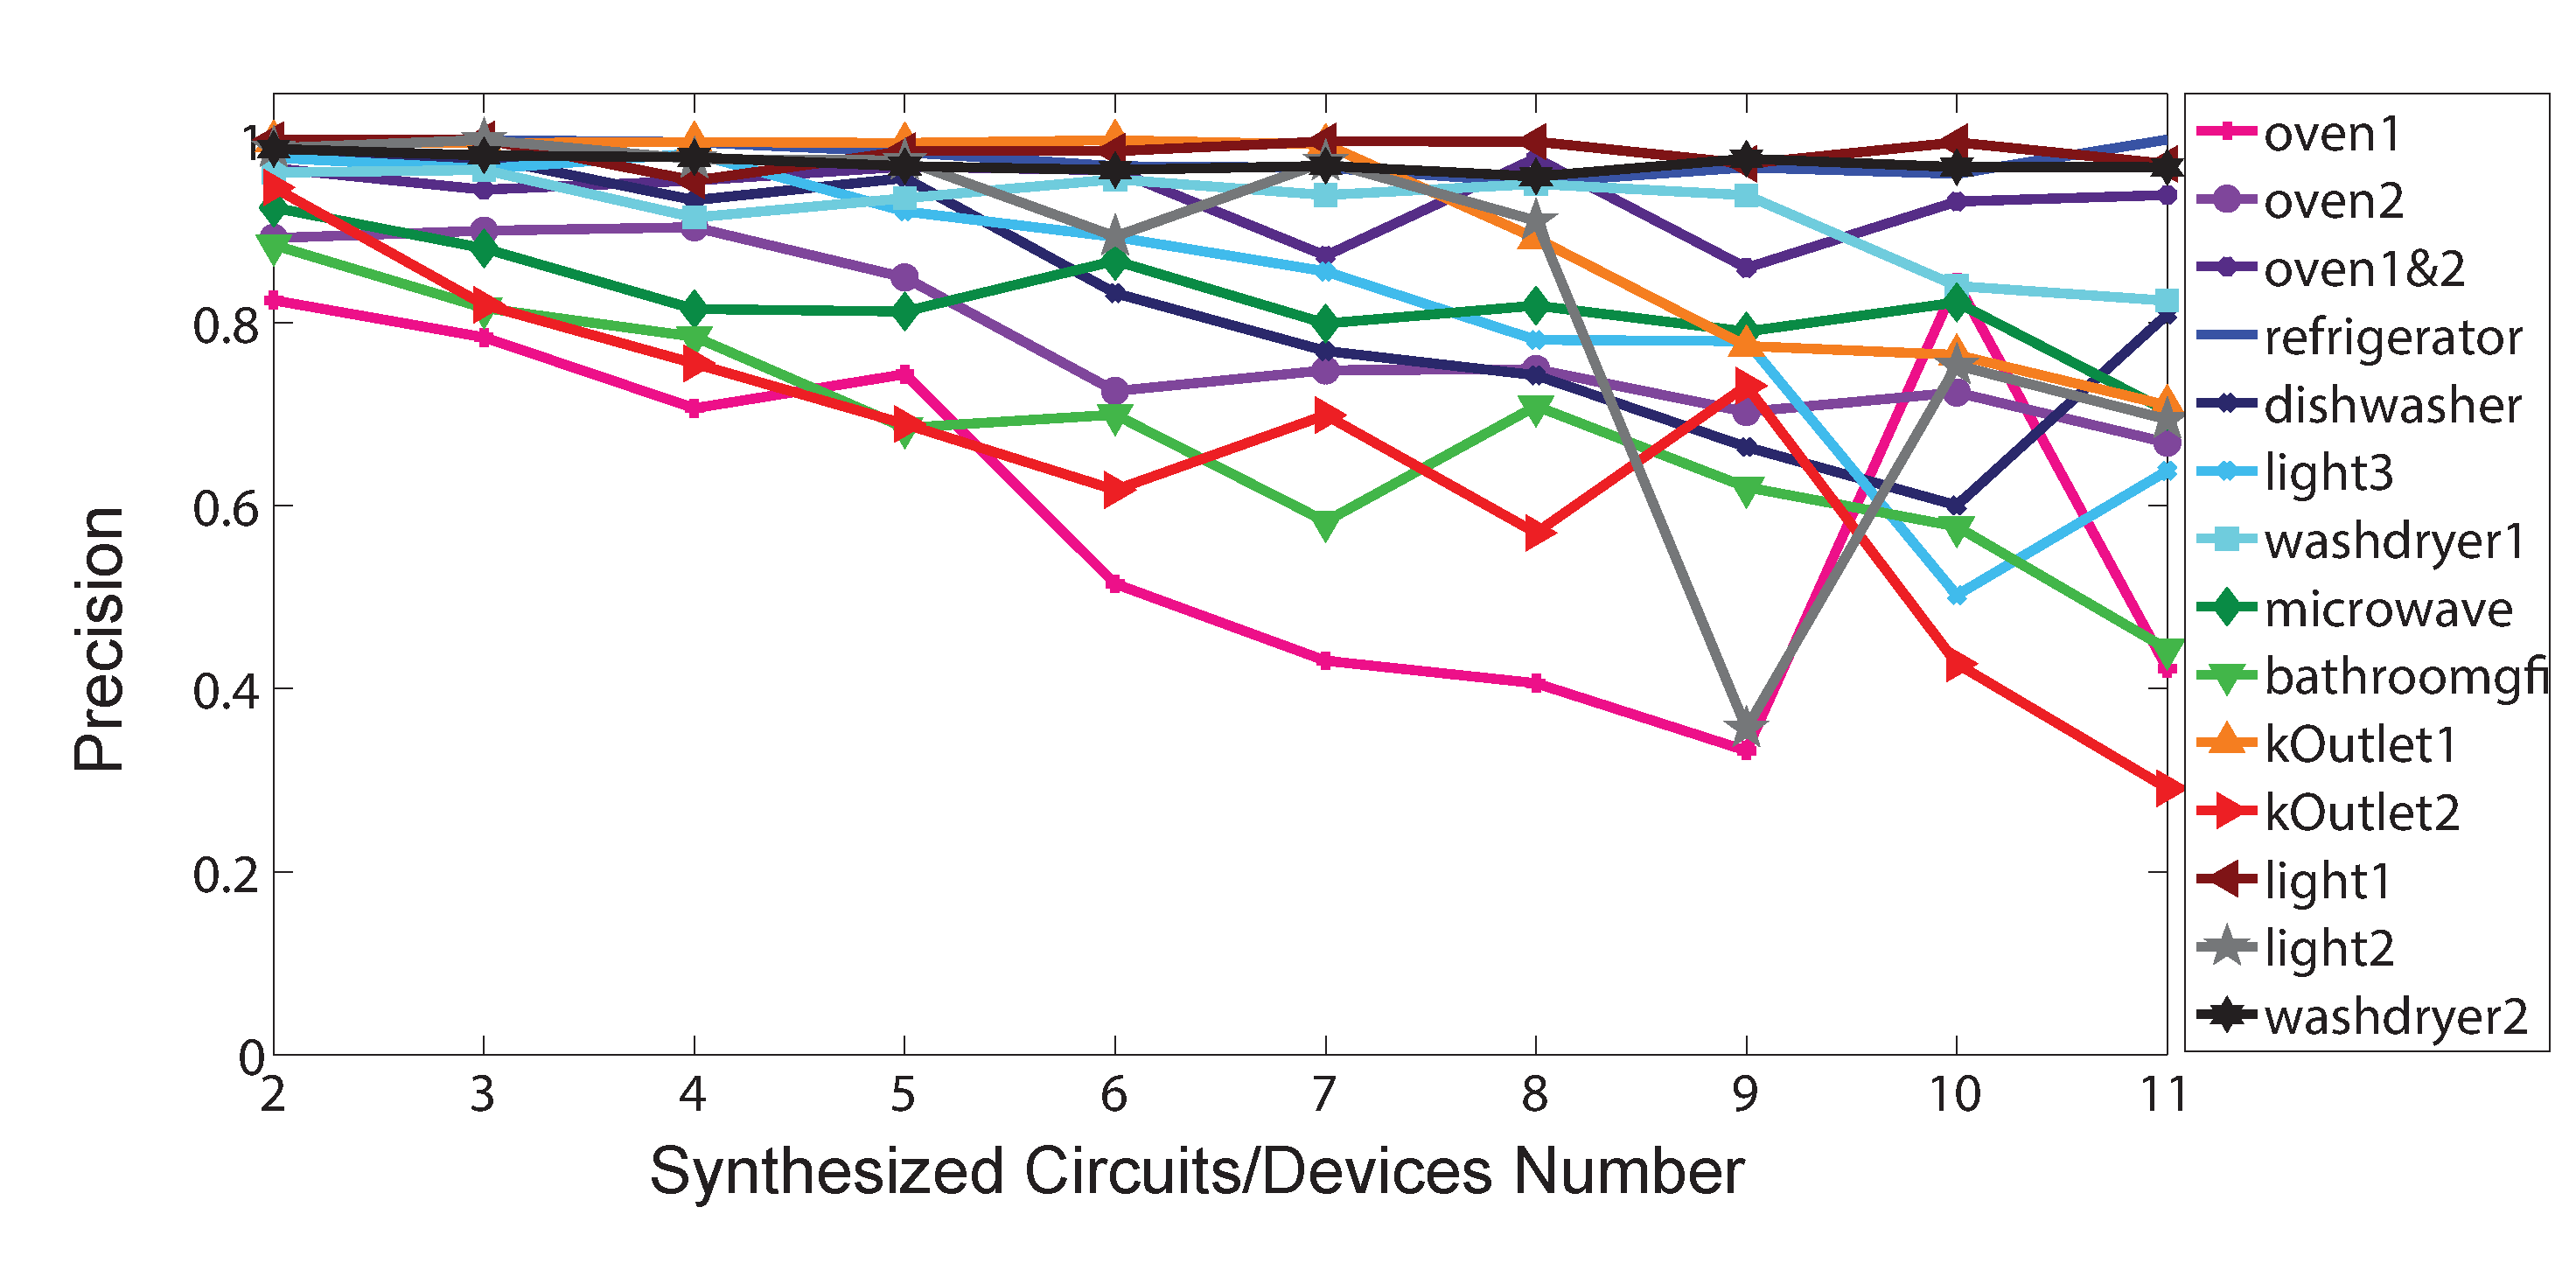
\includegraphics[width=0.49\textwidth]{disaggfigs/14Precisions.pdf} &
		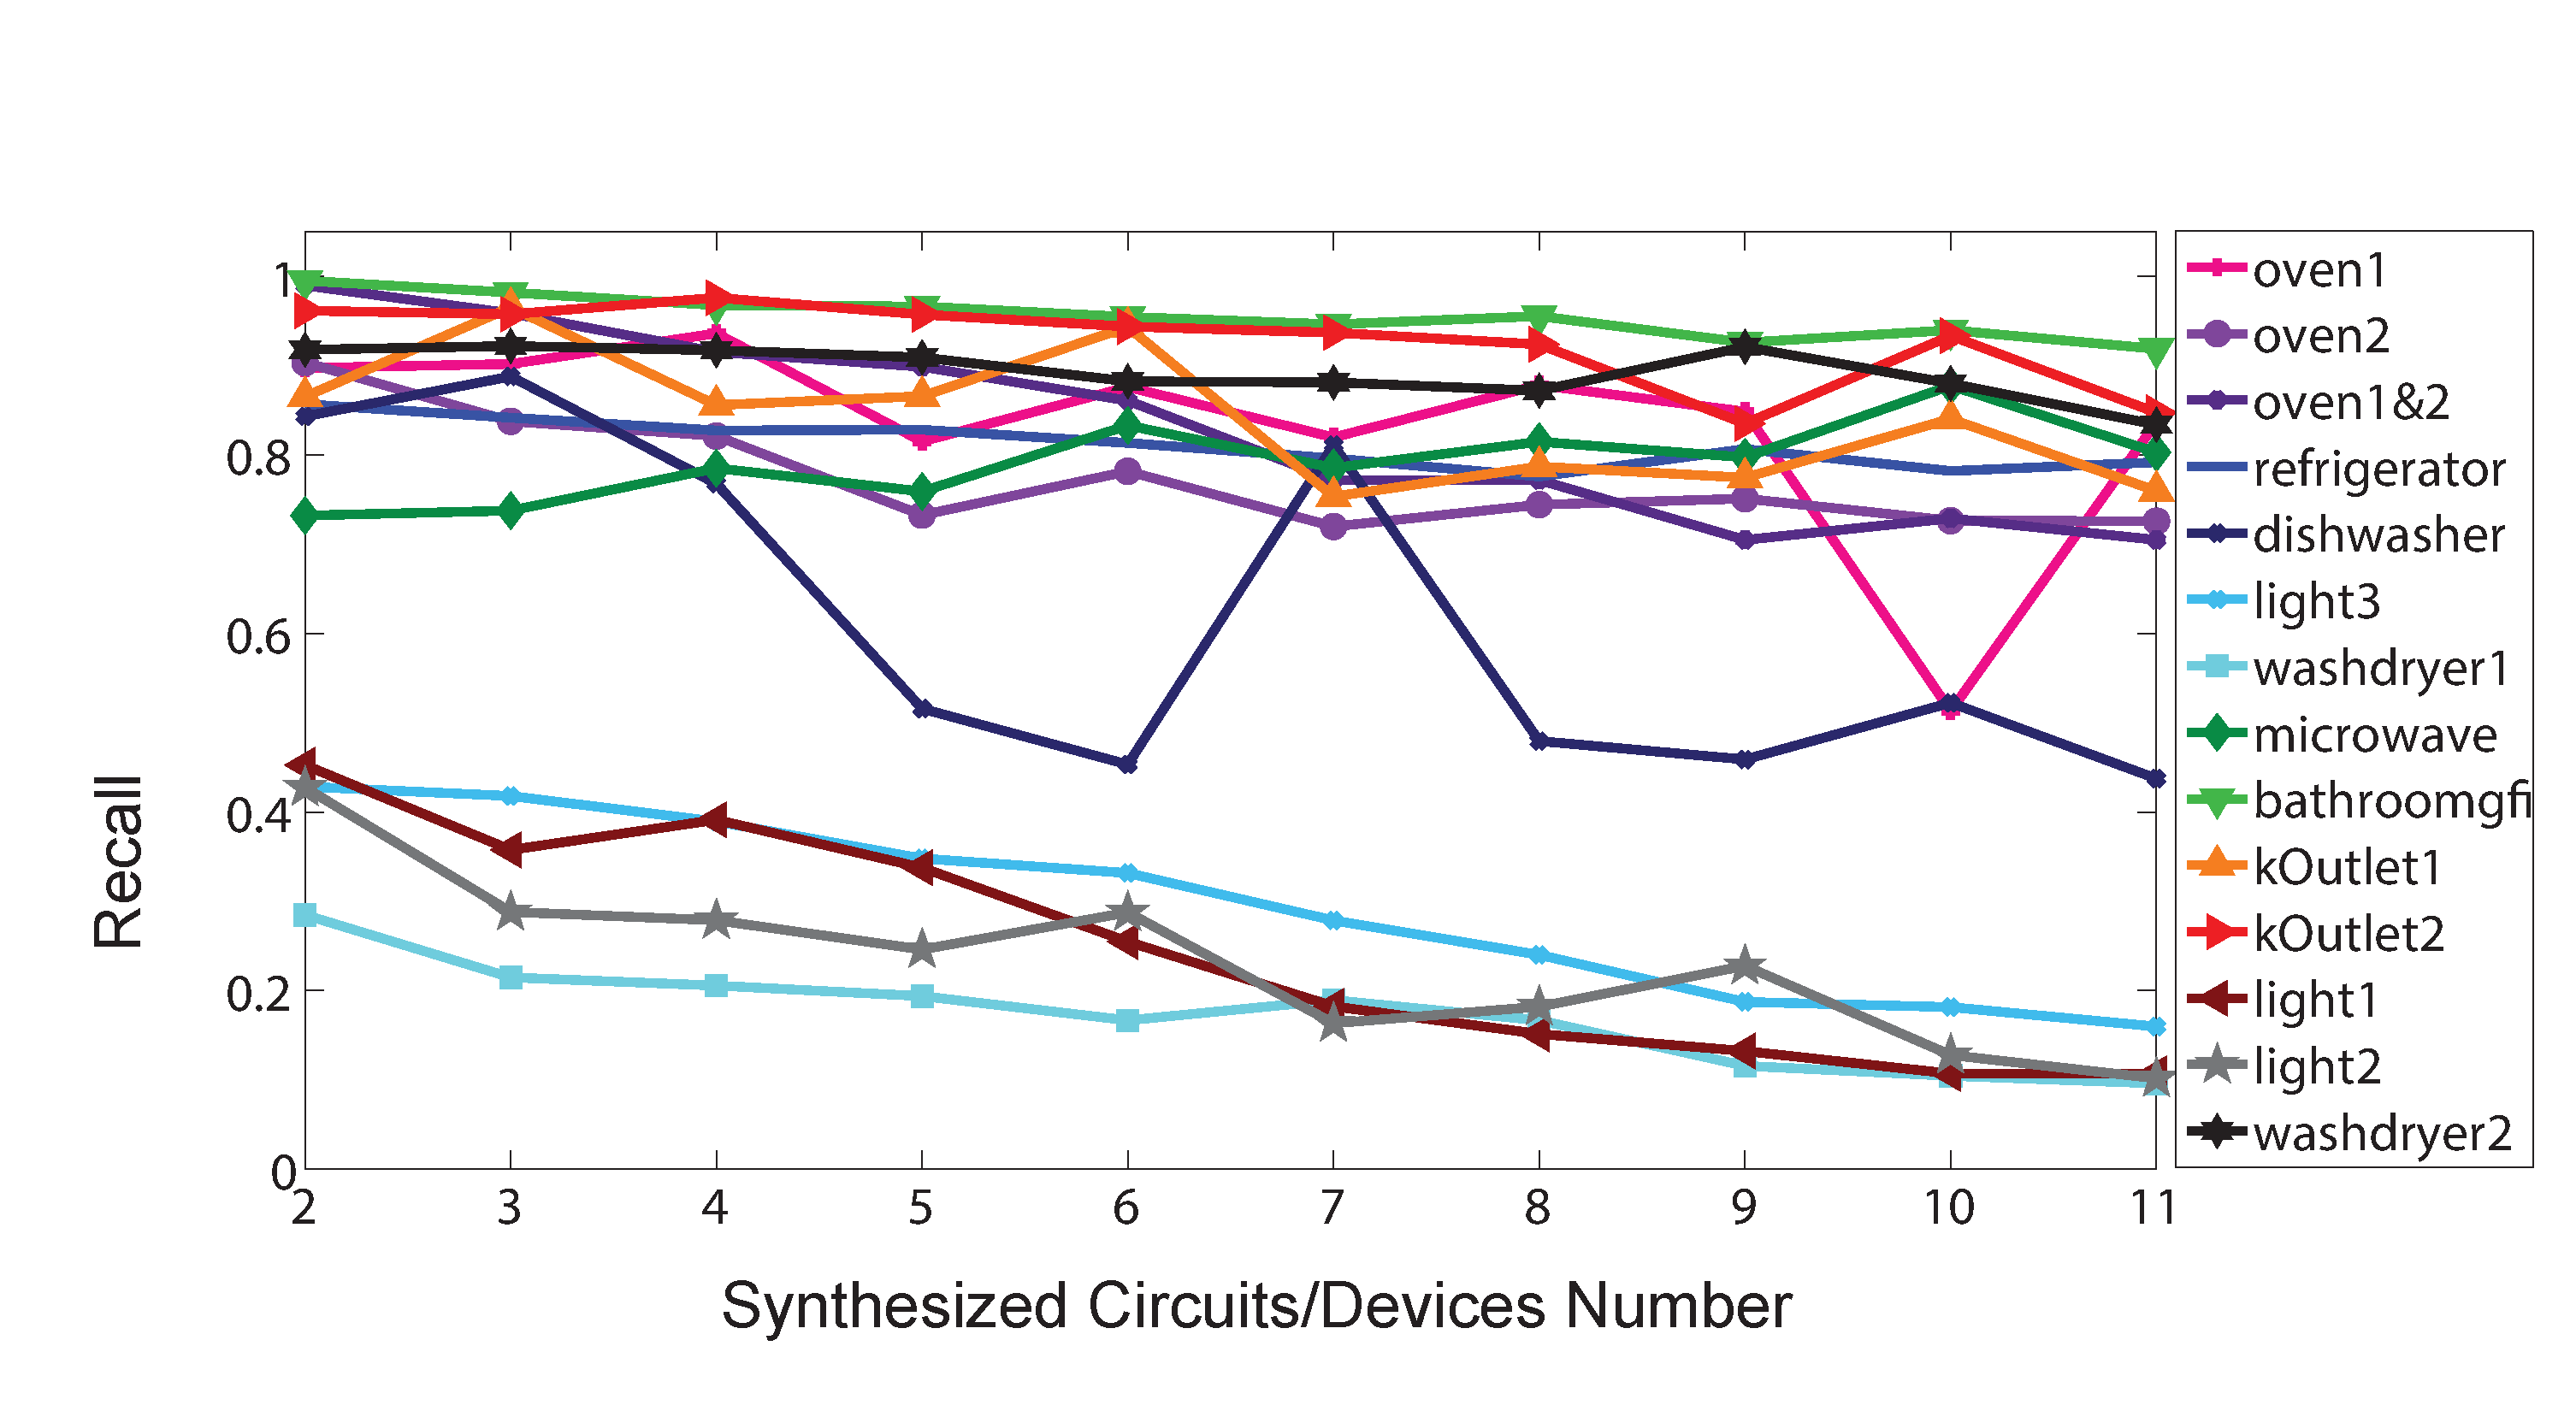
\includegraphics[width=0.49\textwidth]{disaggfigs/14Recalls.pdf}\tabularnewline
		(a) & (b)\tabularnewline
		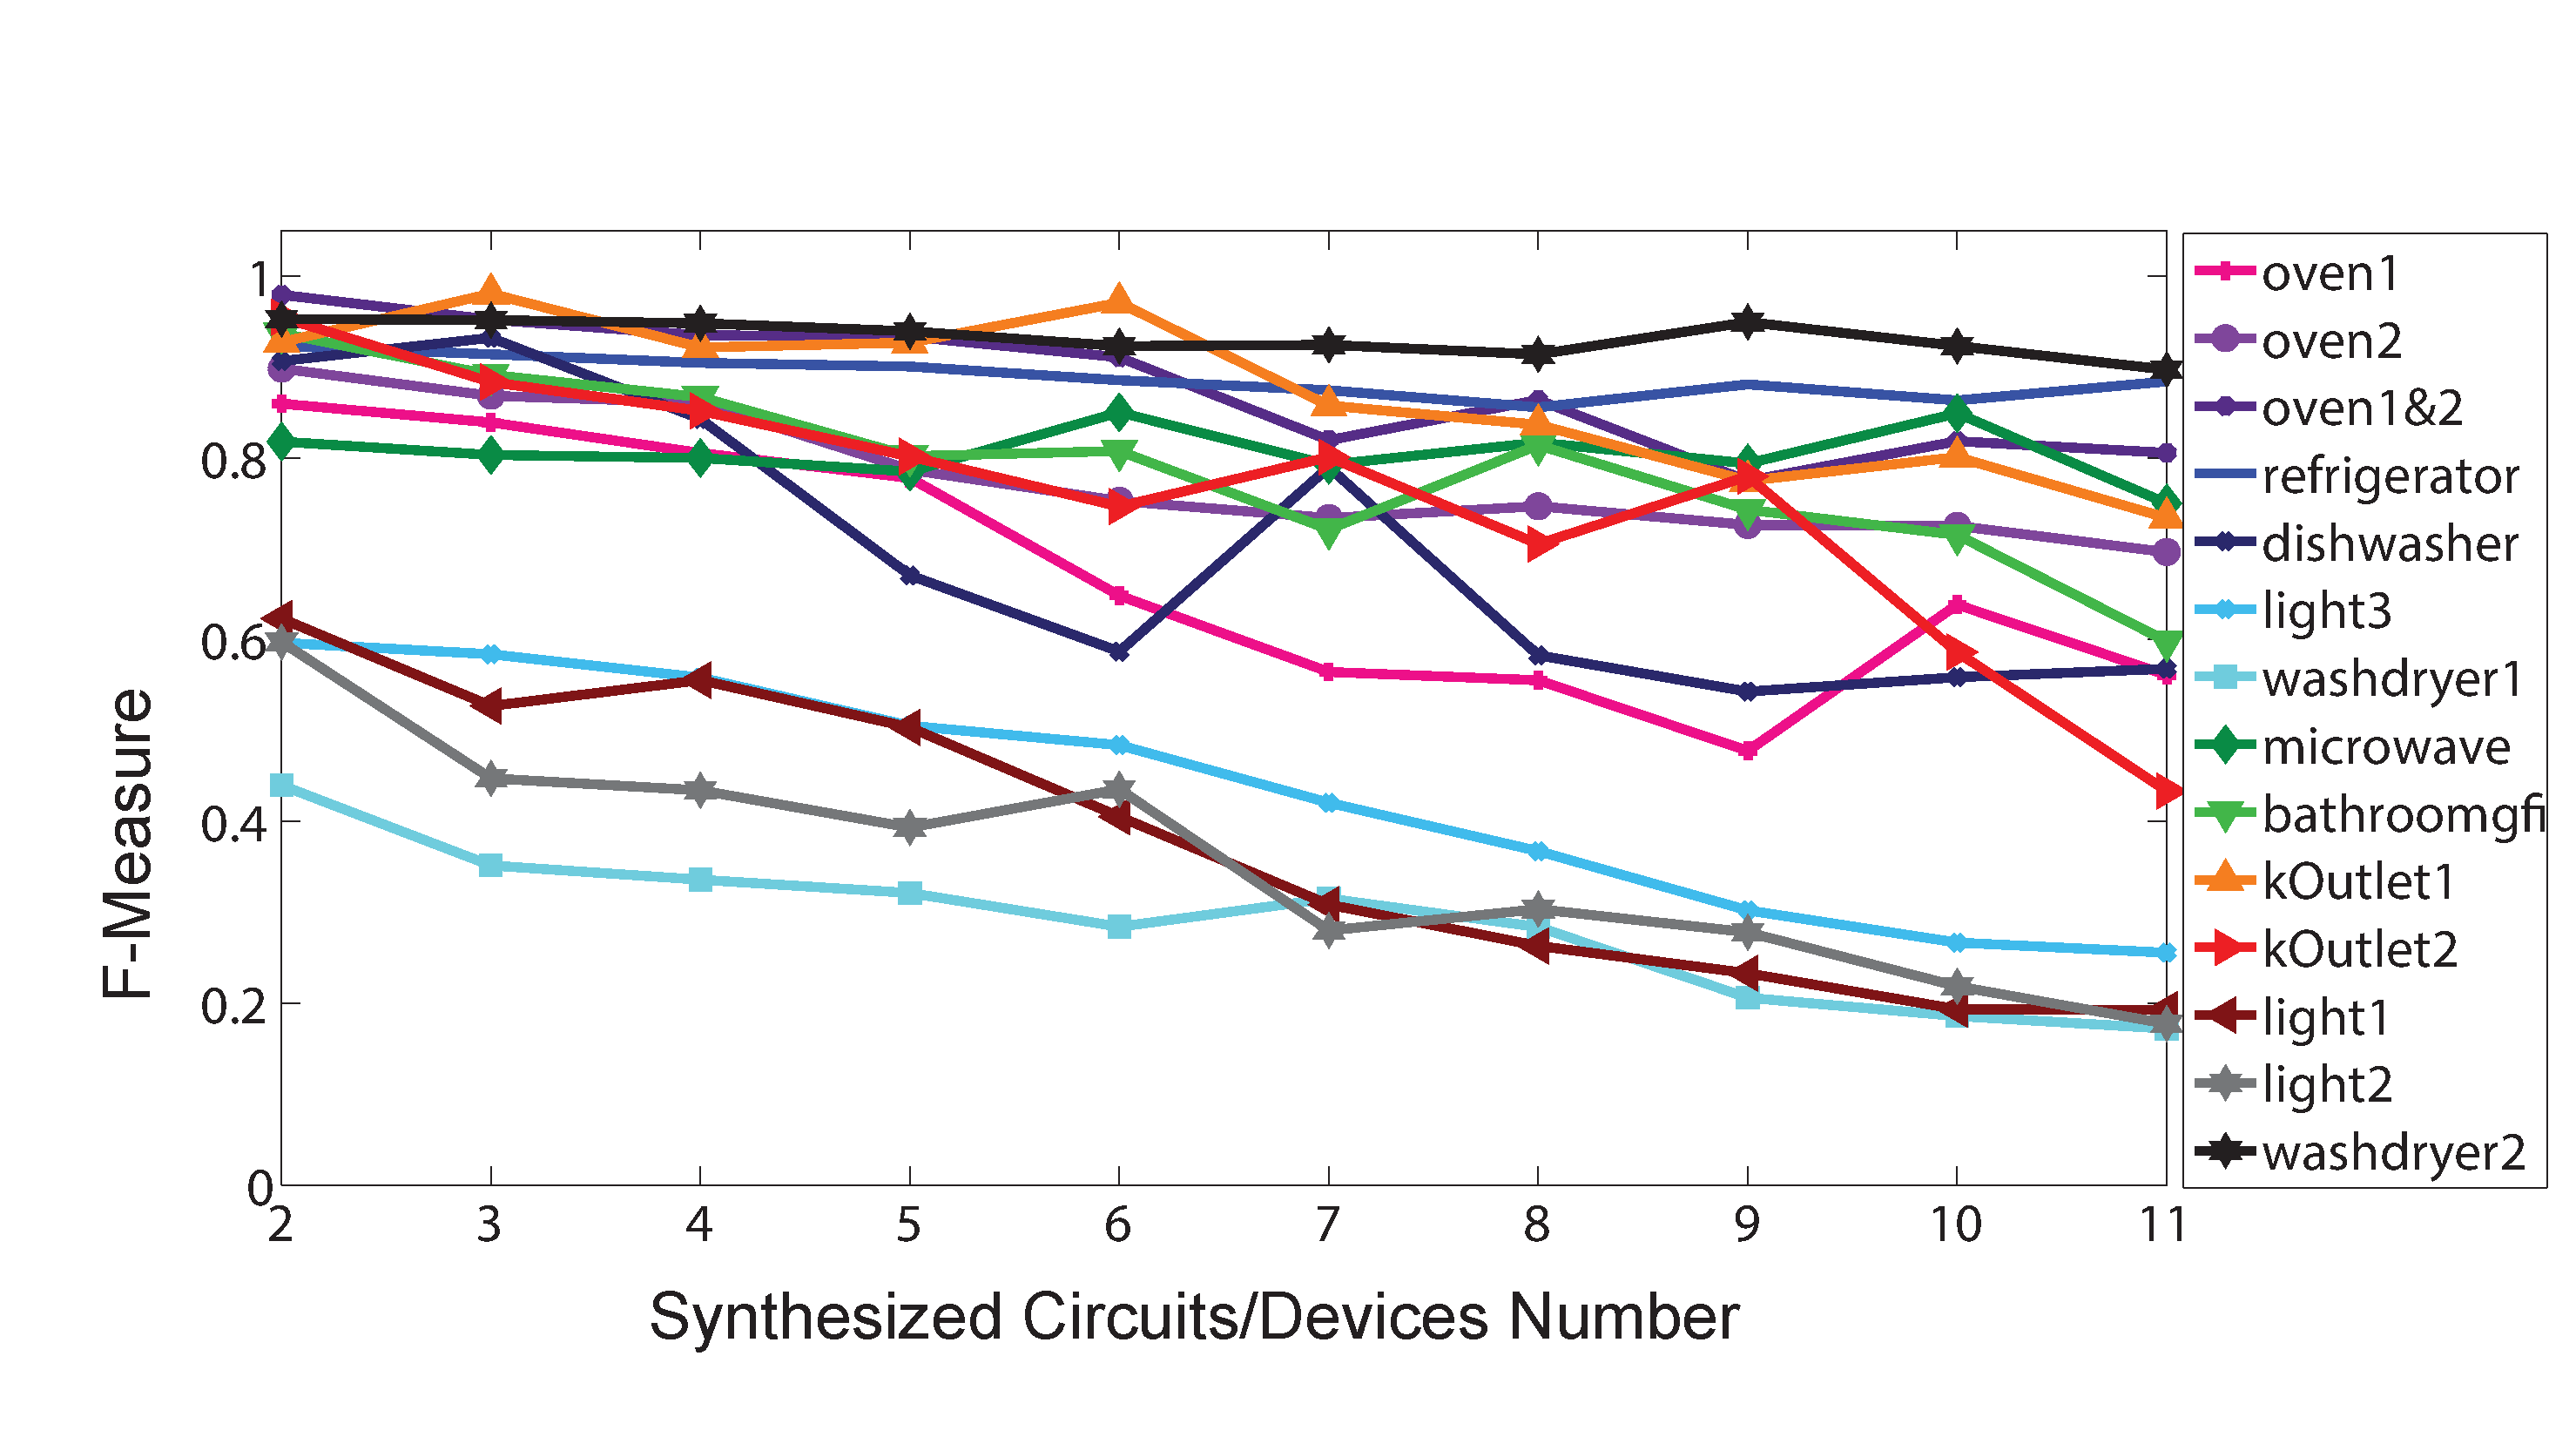
\includegraphics[width=0.49\textwidth]{disaggfigs/14Fmeasures.pdf} &
		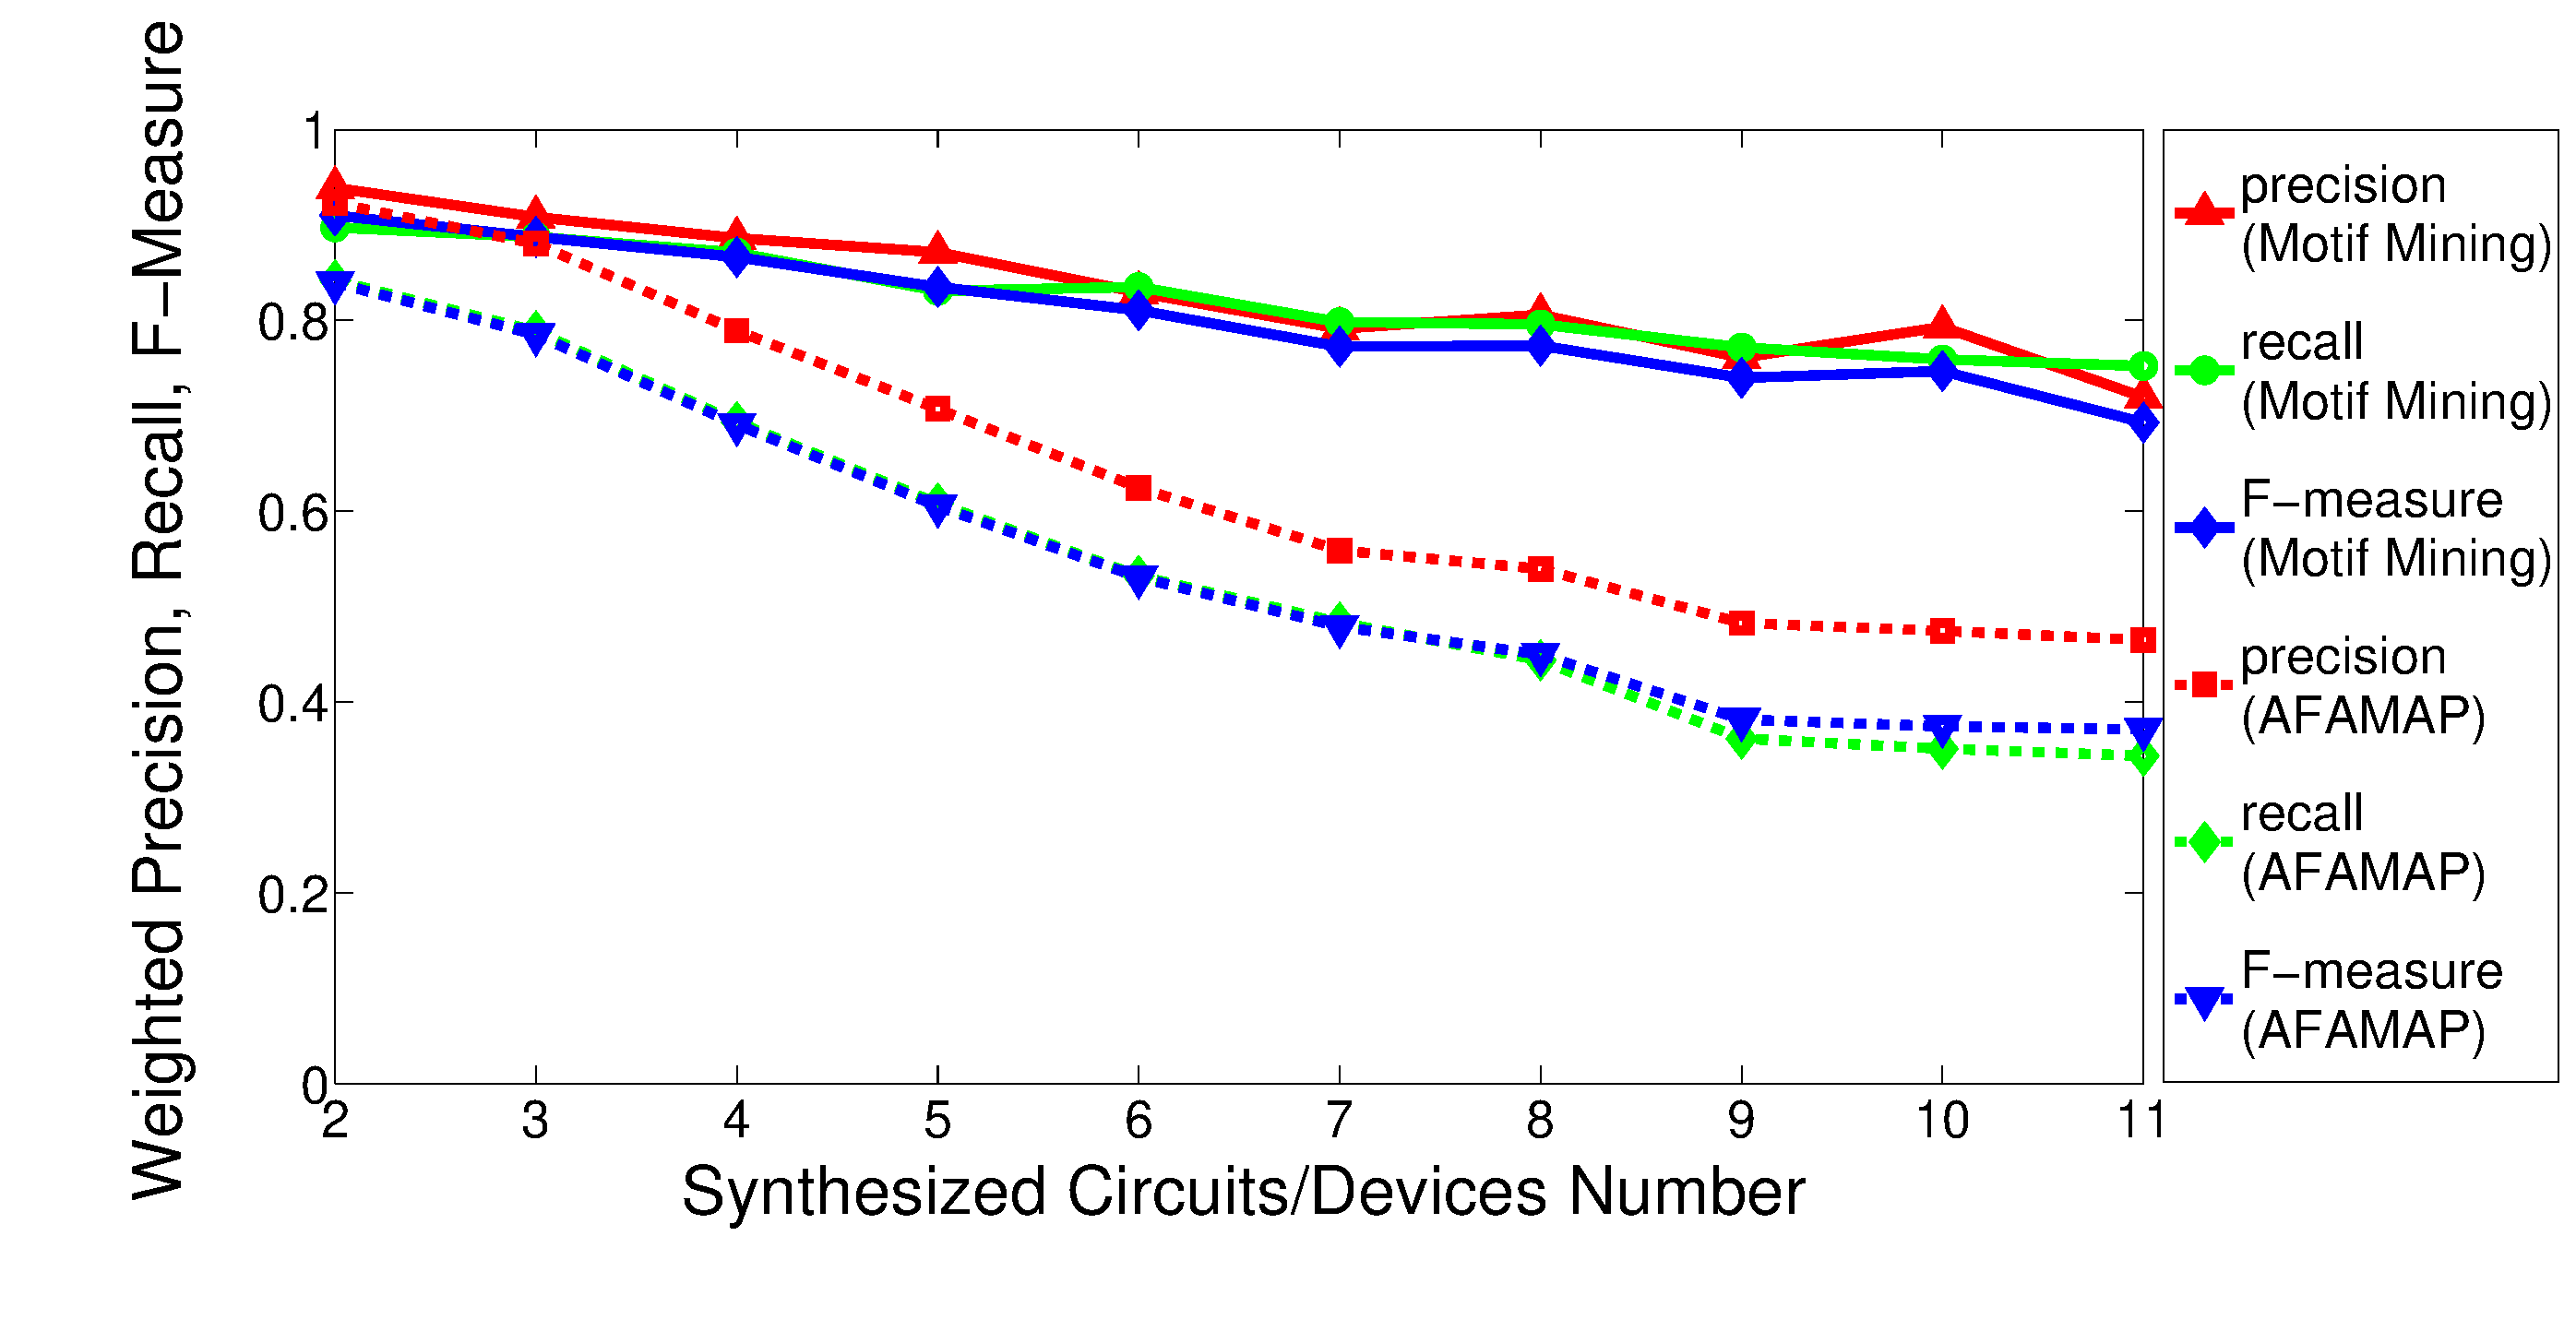
\includegraphics[width=0.49\textwidth]{disaggfigs/weightedPreRecall.pdf} \tabularnewline
		(c) & (d)\tabularnewline
		\end{tabular}
		}
	\caption{
	We increase the number of synthesized circuits from 2 to 11 and
calculate performance measures for disaggregation of each device.
(a) Precision (b) Recall (c) F-measure (d) The precision, recall and F-measure
of all the devices are combined weighed by their average power levels.
}
	\label{fig_synresults}
\end{figure*}

%Figure~\ref{fig_tscmp} illustrates the disaggregation results of 14 devices from 18 devices.
%By comparison, we can see that majority of devices in this period are disaggregated.
%The spikes generated by refrigerator are not reconstructed.
%a portion of time.
%\begin{figure*}[t]
%	\centering{
%    \begin{tabular}{cc}	
%	\includegraphics[width=0.4\textwidth,height=0.2\textheight]{disaggfigs/18truth.pdf} \hspace{1em}&
%    \includegraphics[width=0.4\textwidth,height=0.19\textheight]{disaggfigs/18disagg.pdf} \tabularnewline
%    (a) & (b)\tabularnewline
%    \end{tabular}
%    }
%	\caption{Ground Truth and Disaggregated Circuits}
%	\label{fig_tscmp}
%\end{figure*}

\subsection{Comparison of Motif Mining and AFAMAP}
Next, we conduct experiments comparing our approach with
the AFAMAP algorithm~\cite{kolter2012aistat}, and also
develop a method that combines motif mining and AFAMAP.
Unlike motif mining, AFAMAP requires the power levels of each device;
when running AFAMAP separately, we use the ground truth power levels
for each device. When using AFAMAP in conjunction with motif mining,
we use the power levels from generated episodes as an input to AFAMAP.
Table~\ref{tab_bcmp} lists the results of the comparison.

\begin{table*}[!t]
%\vspace{0.2cm}
\hfill
\begin{minipage}[t]{1.0\linewidth}%
 \centering
\caption {Comparing Motif mining against AFAMAP on the REDD dataset.} \label{tab_bcmp}
%\vspace{0.2cm}
%\begin{center}
\makebox[\textwidth]{\small
\begin{tabular} {|l|p{7mm}|l|l|l|l|l|l|l|l|l|}
\hline
\multirow{2}{*}{device} & True Power (W)& \multicolumn{3}{c|}{Motif mining} & \multicolumn{3}{c|}{AFAMAP (true power levels supplied)}  & \multicolumn{3}{c|}{Motif mining \& AFAMAP}  \\  \cline{3-11}
%\hline
               & &Precision & Recall & F-Measure &  Precision &  Recall & F-Measure & Precision & Recall & F-measure\\
\hline
oven1\&2 &4000& 0.9297 & 0.5209  & 0.6677 &  0.4902 & 0.6750 & 0.5680 &  0.4008 & 0.6708 & 0.5018\\
\hline
refrigerator & 193& 0.9759 & 0.7368 &  0.8396 &0.8825 & 0.3329 & 0.4834 &  0.7791  & 0.5433  & 0.6402  \\
\hline
dishwasher & 1113; 900; 400; 200 &0.9786 & 0.2858 & 0.4423 &0.062 &0.4104 &0.1077 &  0.5337 & 0.7431 & 0.6213  \\
\hline
kOutlets3 & 100; 60&0.1487 &  0.0318 & 0.0524 & 0.6928 & 0.0439 &0.0825 &  0.467 & 0.2892 & 0.3572  \\
\hline
light3 & 282; 90& 0.5768 & 0.1349 & 0.2187 & 0.4396 &0.023 &0.043&  0.5519 & 0.1973 & 0.2907   \\
\hline
washdryer1 & 466; 50& 0.1789 & 0.1236 & 0.1462 & 0.3621 &0.5401 &0.4336 &  0.1703 & 0.6349 & 0.2686  \\
\hline
microwave & 1527& 0.8035 & 0.3799 & 0.5158 &0.5909 &0.2907 &0.3897 &  0.4512 & 0.3741 & 0.4090  \\
\hline
bathroomgfi & 1605& 0.5199 & 0.6815 & 0.5898 & 0.2642 & 0.7551 &0.3915 &  0.1075 & 0.406 & 0.1700   \\
\hline
kOutlet1 & 1076& 0.9320 & 0.6997 & 0.7993 & 0.21 &0.7313 &0.3264&   0.2636 & 0.6394 & 0.3733   \\
\hline
kOutlet 2 &1535 &  0.2233 & 0.6261 & 0.3292 &0.1153 &0.2821 &0.1637 &  0.0234 & 0.0826 & 0.0365  \\
\hline
light1 & 64 & 0.6199 & 0.1963 & 0.2981 & 0.7972 & 0.0796 &0.1447 &  0.667 & 0.1759 & 0.2784  \\
\hline
light2 &53 & 0.2603 &0.1404 &0.1824 &0.6658 &0.0817 &0.1455 &  0.446 & 0.2776 & 0.3422  \\
\hline
washdryer2 &2711 & 0.9563 & 0.8305 & 0.889 & 0.7516 & 0.4237 & 0.5419 &  0.6427 & 0.3301 & 0.4361   \\
\hline
\end{tabular}
%\end{center}
}
\end{minipage}%
%\hfill%
\end{table*}

In all, there are 18 devices but 4 of them are seldom used; and, thus
the remaining 14 devices can be disaggregated by these three methods.
For high power consumption devices, such as oven1\&2, bathroom\_gfi,
kitchen\_outlet1, kitchen\_outlet2 and washdryer2, motif mining performs much better than
AFAMAP even when AFAMAP is supplied with the ground truth power levels.
For some of the low power consumption devices
(such as light1), AFAMAP performs better.
For high frequency devices, such as the refrigerator, motif mining performs much better.

Furthermore, by integrating motif mining and AFAMAP, we see
the performance is much better than the individual algorithms
on multiple state devices such as dishwasher and light3.
Since the power level of light3 is low, the performance
of the integrated method is better than using
only motif mining.

%\input{experimentsComm}
\section{Commercial Building Dataset}
We applied our framework to a
dataset from a commercial building (from HP Labs' campus in Palo Alto, CA).
%(source not provided due to
%double blind review).
Data was collected from a branch in the electrical infrastructure of a large
building and is composed of a root (aggregate) node and seven child
nodes. Although all the nodes are instrumented with meters, we assume only
the root and two of the child nodes, a transformer and a sub-panel, are
available.
The remaining five child nodes are devices that need to be
disaggregated. These are: a pump, a fan, an exhaust fan, a blower, and an
elevator.
The real power of all nodes are logged at intervals of 10 seconds.
Using ground truth data, we combine all five to synthesize the aggregated data.

After the processing steps as described in our framework, we find five power
levels that often occur in a range of just around 1 minute.
Therefore we set the window size to 60 seconds and apply
probabilistic sequential mining using a probability of 0.8 (as described
earlier).
The precision and recall for extracting individual devices is shown in Table~\ref{tab_comm}.

%Until now, we find there are power levels <27kW, -27kW> alone.
%We analyze the occurring time of 27kW and -27kW.
%Surprisedly, 27kW often occurs at 2:10am and
%-27kW happens at 16:20pm on weekday.
%So we employ time-based motif mining to it and
%disaggregate as $Device_3$.
%Those matched episodes with low frequency are discarded.
%
In analyzing these results, we discover that
the baseline power is constituted of two devices, namely,
the pump and the blower.
The elevator shows a sequential episode involving six power levels.
The scheduled device is a fan.
The only un-disaggregated device in our experiments is the exhaust fan
which has very low power consumption compared to others and thus can be disregarded.

\begin{table}
 \centering
\caption {Evaluation measures for commercial building disaggregation.} \label{tab_comm}
%\vspace{0.2cm}
\begin{tabular} {|l|l|l|l|}
\hline
Device& Precision & Recall &F--measure\\
\hline
Pump and blower & 0.99 & 0.99 & 0.99 \\
Fan  & 0.99 & 0.99 & 0.99 \\
Elevator & 0.75 & 0.52 & 0.61  \\
\hline
\end{tabular}
%\end{center}
%\end {table}
%\end{minipage}%
\end{table}

%\section{Conclusion}
Residential occupancy prediction is a hot research topic on controlling the HVAC. 
The accuracy of occupancy prediction influences the comfortability of persons inside 
the home and energy saving. 
In order to achieve the highest prediction result, 
we propose to integrate the mixture EGH model and 
kNN together as a hydrate approach.

Our work differs from previous research based on the main contributions listed below:
\begin{enumerate}
\item We formulate the problem as one of temporal mining: the activities inside the building are abstracted as episodes, and each episode is connected with an episode generative HMM model.
\item We mine the activity patterns according to the time and gap: both the duration of each type of 
activity, and the gap between two consecutive events are limited in a proper range. 
This range is extracted from the historical data according to the weekday and holidays.
\item Our hydrate prediction solution performs best on the workday occupancy prediction: 
in case of normal activities, we apply mixture EGH model; 
in case of abnormal events, we utilize kNN,  
which is generally considered a benchmark in occupancy prediction problem. 
\end{enumerate}
%In this paper, we propose the mixture EGH model and compare it with two other 
%benchmark models, probability density function and kNN approach. 
%The results show that it generally performs better than kNN to predict the 
%occupancy and un-occupancy states in the workdays. 
%The mixture model predicts well for the period of after person getting up and before person 
%going out. 
%The coefficient of the episode generative HMM models helps 
%predict the exact leaving time. 
%However in the case of abnormal events, 
%kNN performs good because it can average the 
%historical data. 
%Even if there is an abnormal day, 
%kNN can leverage it. 

In the future work, we will continue working on the holiday occupancy prediction. 
The occupancy patterns for these days are completely different. 
For example, in certain weekdays, a person may never goes out. 
Therefore the occupancy prediction probably depend more on date other than the indoor activities. 
Further, we will apply this temporal mining approach on the GPS datasets~\cite{koehler2013therml}
to check the effectiveness of occupancy prediction with different kinds of data. 
\section{Discussion}
We have described an intuitive motif-based approach to disaggregation that performs
well relative to more complex algorithms that perform detailed modeling of temporal
profiles.
More importantly,
we have demonstrated how our approach is not just an aid to disaggregation
but, as a byproduct, also extracts temporal episodic relationships that shed
insight into consumption patterns. In this sense, our work goes further
than past work into addressing the real goal of disaggregation research,
namely, to understand systematic trends in consumption patterns with a view
toward identifying opportunities for savings.



%section{ Acknowledgments}
%\newpage
%\clearpage
%\newpage
%\bibliographystyle{aaai}
%\bibliography{references}
%\bigskip

